\documentclass[12pt, a4paper, twoside]{report}

\usepackage{setspace}
\onehalfspacing
%\doublespacing
\usepackage{amsmath, amssymb, amsthm, mathtools,mathrsfs}
\usepackage{pifont}
\allowdisplaybreaks % to break align maths over pages
\usepackage[colorlinks=true, linkcolor=blue, citecolor=blue, backref=page]{hyperref} % backref=page is for backreferencing citations!
\usepackage{bbm, bm}
\usepackage{url}
\usepackage{fancyhdr} %, xspace, psfrag, setspace, supertabular
\usepackage{algorithm, algpseudocode}
\usepackage{graphicx}
\usepackage{geometry} % min OU requirements [inner=40mm, outer=15mm, top=15mm, bottom=20mm]
\usepackage[dvipsnames]{xcolor}
\usepackage{tikz}
\usetikzlibrary{automata,positioning,decorations.pathreplacing, patterns}
\tikzset{>=latex}
\usepackage[procnames]{listings} % Allows inclusion (and syntax highlighting) of C code blocks
\usepackage[font={small}]{caption}
\usepackage{subcaption}
\usepackage{footnote} 
\makesavenoteenv{tabular} % to be able to use footnotes in tabulars
\makesavenoteenv{table} % to be able to use footnotes in tables
\usepackage{stmaryrd} % for averaging operator
\usepackage[utf8]{inputenc}
\usepackage[LGR, T1]{fontenc}
\usepackage{mathdots}
\usepackage{afterpage}

\setlength{\parskip}{1em}

\renewcommand*{\backref}[1]{}
\renewcommand*{\backrefalt}[4]{[{
    \ifcase #1 Not cited.%
          \or Cited on page~#2.%
          \else Cited on pages #2.%
    \fi%
    }]}

\begin{document}



\newtheorem{theorem}{Theorem}[section]
\newtheorem{proposition}{Proposition}[section]
\newtheorem{corollary}{Corollary}[section]
\newtheorem{lemma}{Lemma}[section]
\theoremstyle{definition}
\newtheorem{definition}{Definition}[section]
\newtheorem{example}{Example}[section]
\newtheorem*{note}{Note}
\newtheorem{remark}{Remark}[section]
\newtheorem{observation}{Observation}[section]

\definecolor{keywords}{RGB}{255,0,90}
\definecolor{comments}{RGB}{0,0,113}
\definecolor{myred}{RGB}{160,0,0}
\definecolor{green}{RGB}{0,150,0}


%% For typesetting code listings                                                
\lstdefinelanguage{Sage}[]{Python}
{morekeywords={False,sage,True},sensitive=true}
\newcommand{\lstsetsage}{\lstset{
  frame=single,
  showtabs=False,
  showspaces=False,
  showstringspaces=False,
  commentstyle={\ttfamily\color{dgraycolor}},
  keywordstyle={\ttfamily\color{dbluecolor}\bfseries},
  stringstyle={\ttfamily\color{dgreencolor}\bfseries},
  language=Sage,
  basicstyle={\fontsize{9pt}{9pt}\ttfamily},
  aboveskip=0.3em,
  belowskip=0.1em,
  numbers=left,
  numberstyle=\tiny
}}

\newcommand{\lstsetbash}{\lstset{
    language=bash,
    basicstyle={\fontsize{9pt}{9pt}\ttfamily},
    deletekeywords={local, for, help},
    keywordstyle=\color{keywords},
    commentstyle=\color{comments},
    stringstyle=\color{black},
    numbers=none,
    stepnumber=1,
    frame=single,
    showstringspaces=false,
}}

\definecolor{dblackcolor}{rgb}{0.0,0.0,0.0}
\definecolor{dbluecolor}{rgb}{0.01,0.02,0.7}
\definecolor{dgreencolor}{rgb}{0.2,0.4,0.0}
\definecolor{dgraycolor}{rgb}{0.30,0.3,0.30}
\newcommand{\dblue}{\color{dbluecolor}\bf}
\newcommand{\dred}{\color{dredcolor}\bf}
\newcommand{\dblack}{\color{dblackcolor}\bf}


\newcommand{\shellcmd}[1]{\texttt{\footnotesize\$ #1}}
\renewcommand{\vert}[1]{\ensuremath{\llbracket #1 \rrbracket}} % Razborov's averaging operator
\newcommand{\Av}{\ensuremath{\mathrm{Av}}}
\newcommand{\Si}{\ensuremath{\mathrm{Si}}}
\newcommand{\seq}[1]{\text{\textsc{Seq}}[#1]}
\newcommand{\D}[1]{\ensuremath{\mathrm{\textbf{D}}}}
\renewcommand{\P}{\ensuremath{\mathcal{P}}}
\newcommand{\T}{\ensuremath{\mathcal{T}}}
\newcommand{\V}{\ensuremath{\mathcal{V}}}
\newcommand{\B}{\ensuremath{\mathcal{B}}}
\newcommand{\Z}{\ensuremath{\mathcal{Z}}}
\newcommand{\Zstar}{\ensuremath{\mathcal{Z}^*}}
\newcommand{\M}{\ensuremath{\mathcal{M}}}
\newcommand{\Mstar}{\ensuremath{\mathcal{M}^*}}
\newcommand{\barMstar}{\ensuremath{\overline{\mathcal{M}}^*}}
\newcommand{\EE}{\ensuremath{\mathcal{E}}}
\newcommand{\C}{\ensuremath{\mathcal{C}}}
\newcommand{\Cstar}{\ensuremath{\mathcal{C}^*}}
\newcommand{\HH}{\ensuremath{\mathcal{H}}}
\newcommand{\HHstar}{\ensuremath{\mathcal{H}^*}}
\newcommand{\hatC}{\ensuremath{\widehat{\mathcal{C}}}}
\newcommand{\hatCstar}{\ensuremath{\widehat{\mathcal{C}}^*}}
\newcommand{\barC}{\ensuremath{\overline{\mathcal{C}}}}
\newcommand{\barCstar}{\ensuremath{\overline{\mathcal{C}}^*}}
\newcommand{\Q}{\ensuremath{\mathcal{Q}}}
\newcommand{\F}{\ensuremath{\mathcal{F}}}
\renewcommand{\S}{\ensuremath{\mathcal{S}}}
\newcommand{\Sstar}{\ensuremath{\mathcal{S}^*}}
\renewcommand{\SS}{\ensuremath{\mathbb{S}}}
\newcommand{\rS}{\ensuremath{\mathscr{S}}}
\newcommand{\DD}{\ensuremath{\mathcal{D}}}
\newcommand{\DDstar}{\ensuremath{\mathcal{D}^*}}
\newcommand{\RR}{\ensuremath{\mathbb{R}}}

% Serif font
\newcommand{\fL}{\ensuremath{\mathsf{L}}}
\newcommand{\fR}{\ensuremath{\mathsf{R}}}
\newcommand{\fD}{\ensuremath{\mathsf{D}}}
\newcommand{\fU}{\ensuremath{\mathsf{U}}}
\newcommand{\fC}{\ensuremath{\mathsf{C}}}
\newcommand{\fB}{\ensuremath{\mathsf{B}}}
\newcommand{\fS}{\ensuremath{\mathsf{S}}}
\newcommand{\fM}{\ensuremath{\mathsf{M}}}
\newcommand{\fE}{\ensuremath{\mathsf{E}}}
\newcommand{\fX}{\ensuremath{\mathsf{X}}}

% bold Serif font
\newcommand{\bD}{\ensuremath{\textbf{\textsf{D}}}}
\newcommand{\bU}{\ensuremath{\textbf{\textsf{U}}}}
\newcommand{\bC}{\ensuremath{\textbf{\textsf{C}}}}
\newcommand{\bE}{\ensuremath{\textbf{\textsf{E}}}}
\newcommand{\bbU}{\ensuremath{\mathbb{U}}}
\newcommand{\bM}{\ensuremath{\textbf{\textsf{M}}}}
\renewcommand{\bm}{\ensuremath{\mathbf{m}}}
\newcommand{\bc}{\ensuremath{\mathbf{c}}}
\newcommand{\be}{\ensuremath{\mathbf{e}}}

\newcommand{\distav}[2]{\ensuremath{\mathbb{A}_{#1}(#2)}}
\newcommand{\N}{\ensuremath{\mathbb{N}}}
\newcommand{\rhs}{\ensuremath{\mathrm{RHS}}}
\newcommand{\lhs}{\ensuremath{\mathrm{LHS}}}
\newcommand{\argmax}[1]{\ensuremath{\mathrm{argmax}(#1)}}
\newcommand{\argmin}[1]{\ensuremath{\mathrm{argmin}(#1)}}
\newcommand{\Prob}[1]{\ensuremath{\mathbf{Pr}\left(#1\right)}}
\newcommand{\E}[1]{\ensuremath{\mathbf{E}\left(#1\right)}}
\newcommand{\Exp}[2]{\ensuremath{\mathbf{E}_{#1}\left(#2\right)}}
\newcommand{\1}[1]{\ensuremath{\mathbbm{1}_{#1}}}
\newcommand{\2}[2]{\ensuremath{\mathbbm{1}_{#1}\left(#2\right)}}
\newcommand{\Space}{\ensuremath{\mathcal{S}}}
\newcommand{\powerset}[1]{\ensuremath{\mathcal{P}\left(#1\right)}}
\newcommand{\mg}[1]{\ensuremath{\mathrm{mg}\left(#1\right)}}
\newcommand{\gr}[1]{\ensuremath{\mathrm{gr}\left(#1\right)}}
\newcommand{\ugr}[1]{\ensuremath{\overline{\mathrm{gr}}\left(#1\right)}}
\newcommand{\ex}{\ensuremath{\mathrm{ex}}}
\newcommand{\im}{\ensuremath{\mathrm{im}}}
\newcommand{\bigominus}{\ensuremath{\mathlarger{\mathlarger{\mathlarger{\ominus}}}}}
\newcommand{\x}{\ensuremath{\mathbf{x}}}
\newcommand{\Grid}{\ensuremath{\mathrm{Grid}}}


%%%%%%%%%%%%%%%%%%%%%%%%%%%%%%%%%%%%%%%%%
% DYCK PATHS
%%%%%%%%%%%%%%%%%%%%%%%%%%%%%%%%%%%%%%%%%


% drawing Dyck paths:
\newcommand\dyck[4]{
  % start point, size, Dyck word (size x 2 booleans)
  \fill[white]  (#1) rectangle +(#2,#2);
  \draw[help lines] (#1) grid +(#2,#2);
  %\draw[dashed] (#1) -- +(#2,#2);
  \coordinate (prev) at (#1);
  \foreach \dir in {#4}{
    \ifnum\dir=0
    \coordinate (dep) at (1,0);
    \else
    \coordinate (dep) at (0,1);
    \fi
    \draw[line width=2pt, color=#3, cap=round] (prev) -- ++(dep) coordinate (prev);
  };
}


% drawing Dyck paths without grid
\newcommand\pdyck[3]{
  % start point, size, Dyck word (size x 2 booleans)
  \coordinate (prev) at (#1);
  \foreach \dir in {#3}{
    \ifnum\dir=0
    \coordinate (dep) at (1,0);
    \else
    \coordinate (dep) at (0,1);
    \fi
    \draw[line width=2pt, color=#2, cap=round, style=dotted] (prev) -- ++(dep) coordinate (prev);
  };
}


%%%%%%%%%%%%%%%%%%%%%%%%%%%%%%%%%%%%%%%%%%
% CONSTRUCTIONS OF PERMUTONS
%%%%%%%%%%%%%%%%%%%%%%%%%%%%%%%%%%%%%%%%%%
\newcommand{\acbmax}{
  \begin{tikzpicture}[scale=0.5]
    \draw (0,1.7)--(1.3,3);
    \draw (1.3,1)--(2,1.7);
    \draw (2,0.7)--(2.3,1);
    \draw (2.3,0.5)--(2.5,0.7);
    \draw (2.5,0.4)--(2.6,0.5);
    \draw (2.65,0.3)--(2.7,0.35);
  \end{tikzpicture}}


\newcommand{\acdbmax}{
  \begin{tikzpicture}[scale=0.4]

    %\node at (-8,0) {$\Gamma\ = $};
    \draw (3,6)--(5,8);
    \draw (5,4.7)--(6.3,6);
    \draw (6.3,4)--(7,4.7);
    \draw (7,3.7)--(7.3,4);
    \draw (7.3,3.5)--(7.5,3.7);
    \draw (7.5,3.4)--(7.6,3.5);
    \draw (7.65,3.3)--(7.7,3.35);

    \draw (0,1.7)--(1.3,3);
    \draw (1.3,1)--(2,1.7);
    \draw (2,0.7)--(2.3,1);
    \draw (2.3,0.5)--(2.5,0.7);
    \draw (2.5,0.4)--(2.6,0.5);
    \draw (2.65,0.3)--(2.7,0.35);

    \draw (-1.7,-0.7)--(-1,0);
    \draw (-1,-1)--(-0.7,-0.7);
    \draw (-0.7,-1.2)--(-0.5,-1);
    \draw (-0.5,-1.3)--(-0.4,-1.2);
    \draw (-0.35,-1.4)--(-0.3,-1.35);

    \draw (-2.7,-2.3)--(-2.4,-2);
    \draw (-2.4,-2.5)--(-2.2,-2.3);
    \draw (-2.2,-2.6)--(-2.1,-2.5);
    \draw (-2.05,-2.7)--(-2,-2.65);

    \draw[thick] (-3.05,-3.05)--(-3,-3);
    \draw[thick] (-3.25,-3.25)--(-3.2,-3.2);
    \draw[thick] (-3.45,-3.45)--(-3.4,-3.4);


    \draw (14,2)--(16,2);
    \draw (14,1.5)--(16,1.5);

    \draw (25,6)--(27,8)--(29.7,3.35)--(25,6);
    \draw (20,-2.35)--(25,-2.35)--(25,3.35)--(20,3.35)--(20,-2.35);

  \end{tikzpicture}}






\newcommand{\Amax}{
  \begin{tikzpicture}[baseline=1ex, scale=0.15]
    \draw (0,1.7)--(1.3,3);
    \draw (1.3,1)--(2,1.7);
    \draw (2,0.7)--(2.3,1);
    \draw (2.3,0.5)--(2.5,0.7);
    \draw (2.5,0.4)--(2.6,0.5);
    \draw (2.65,0.3)--(2.7,0.35);

    \draw (3,5)--(5,3);
  \end{tikzpicture}}

\newcommand{\AAmax}{
  \begin{tikzpicture}[baseline=1ex, scale=0.15]
    \draw (0,1.7)--(1.3,3);
    \draw (1.3,1)--(2,1.7);
    \draw (2,0.7)--(2.3,1);
    \draw (2.3,0.5)--(2.5,0.7);
    \draw (2.5,0.4)--(2.6,0.5);
    \draw (2.65,0.3)--(2.7,0.35);

    \draw (2.5,5)--(5,2.5);
  \end{tikzpicture}}




\newcommand{\Bmax}{
  \begin{tikzpicture}[baseline=1ex, scale=0.15]
    \draw (3,3)--(5,5);
    \draw (5,1)--(7,3);

    \draw (1,0)--(2,1);
    \draw (2,-1)--(3,0);
    
    \draw (0,-1.5)--(0.5,-1);
    \draw (0.5,-2)--(1,-1.5);

    \draw (-0.4,-2.2)--(-0.2,-2);
    \draw (-0.2,-2.4)--(0,-2.2);

  \end{tikzpicture}}



\newcommand{\Cmax}{
  \begin{tikzpicture}[baseline=1ex, scale=0.15]

    \draw (3,5)--(5,3);
    \draw (2,3)--(3,2);
    \draw (1,2)--(2,1);
    \draw (-1,1)--(1,-1);
  \end{tikzpicture}}




\newcommand{\Dmax}{
  \begin{tikzpicture}[baseline=1ex, scale=0.15]
    \draw (0,1.7)--(1.3,3);
    \draw (1.3,1)--(2,1.7);
    \draw (2,0.7)--(2.3,1);
    \draw (2.3,0.5)--(2.5,0.7);
    \draw (2.5,0.4)--(2.6,0.5);
    \draw (2.65,0.3)--(2.7,0.35);

    \draw (3,4.7)--(4.3,6);
    \draw (4.3,4)--(5,4.7);
    \draw (5,3.7)--(5.3,4);
    \draw (5.3,3.5)--(5.5,3.7);
    \draw (5.5,3.4)--(5.6,3.5);
    \draw (5.65,3.3)--(5.7,3.35);
  \end{tikzpicture}}

\newcommand{\Dmaxr}{
  \begin{tikzpicture}[baseline=1ex, scale=0.15]
    \draw (0,1.7)--(1.3,3);
    \draw (1.3,1)--(2,1.7);
    \draw (2,0.7)--(2.3,1);
    \draw (2.3,0.5)--(2.5,0.7);
    \draw (2.5,0.4)--(2.6,0.5);
    \draw (2.65,0.3)--(2.7,0.35);

    \draw (4.5,3)--(5.8,4.3);
    \draw (3.8,4.3)--(4.5,5);
    \draw (3.5,5)--(3.8,5.3);
    \draw (3.3,5.3)--(3.5,5.5);
    \draw (3.2, 5.5)--(3.3, 5.6);
    \draw (3.15, 5.6)--(3.2, 5.65);
  \end{tikzpicture}}


\newcommand{\Emax}{
  \begin{tikzpicture}[baseline=1ex, scale=0.15]

    \draw (0,2)--(2,0);
    \draw (2,4)--(4,6);
    \draw (4,2)--(6,4);
  \end{tikzpicture}}



% 1342 7term
\newcommand{\acdbmaxapprox}{
  \begin{tikzpicture}[baseline=1ex, scale=0.5]
    \draw (0,1.7)--(1.3,3);
    \draw (1.3,1)--(2,1.7);
    \draw (2,0.7)--(2.3,1);
    \draw (2.3,0.5)--(2.5,0.7);
    \draw (2.5,0.4)--(2.6,0.5);
    \draw (2.65,0.3)--(2.7,0.35);
  \end{tikzpicture}}


%%%%%%%%%%%%%%%%%%%%%%%%%%%%%%%%%%%%%%%%%%%%
% SMALL PERMUTATION PICTOGRAMS
%%%%%%%%%%%%%%%%%%%%%%%%%%%%%%%%%%%%%%%%%%%%

\newcommand{\dicycle}{
  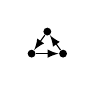
\begin{tikzpicture}[baseline=-0.3ex,scale=0.2]
    \tikzstyle{vertex}=[circle,fill=black, minimum size=1pt,inner sep=1pt]
    \node[vertex] (v1) at (0,0){};
    \node[vertex] (v2) at (2,0){};
    \node[vertex] (v3) at (1,1.4){};
    \draw[->](v1)--(v2);
    \draw[->](v2)--(v3);
    \draw[->](v3)--(v1);
  \end{tikzpicture}
}

\newcommand{\twochain}{
  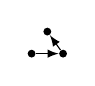
\begin{tikzpicture}[baseline=-0.3ex,scale=0.2]
    \tikzstyle{vertex}=[circle,fill=black, minimum size=1pt,inner sep=1pt]
    \node[vertex] (v1) at (0,0){};
    \node[vertex] (v2) at (2,0){};
    \node[vertex] (v3) at (1,1.4){};
    \draw[->](v1)--(v2);
    \draw[->](v2)--(v3);
  \end{tikzpicture}
}

\newcommand{\orcocherry}{
  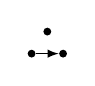
\begin{tikzpicture}[baseline=-0.3ex,scale=0.2]
    \tikzstyle{vertex}=[circle,fill=black, minimum size=1pt,inner sep=1pt]
    \node[vertex] (v1) at (0,0){};
    \node[vertex] (v2) at (2,0){};
    \node[vertex] (v3) at (1,1.4){};
    \draw[->](v1)--(v2);
  \end{tikzpicture}
}

\newcommand{\outstar}{
  
\begin{tikzpicture}[baseline=-0.3ex,scale=0.2]
    \tikzstyle{vertex}=[circle,fill=black, minimum size=1pt,inner sep=1pt]
    \node[vertex] (v1) at (0,0){};
    \node[vertex] (v2) at (2,0){};
    \node[vertex] (v3) at (1,1.4){};
    \draw[->](v3)--(v1);
    \draw[->](v3)--(v2);
  \end{tikzpicture}
}


\newcommand{\digraphacbd}{
  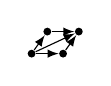
\begin{tikzpicture}[baseline=-0.3ex,scale=0.2]
    \tikzstyle{vertex}=[circle,fill=black, minimum size=1pt,inner sep=1pt]
    \node[vertex] (v1) at (0,0){};
    \node[vertex] (v2) at (2,0){};
    \node[vertex] (v3) at (1,1.4){};
    \node[vertex] (v4) at (3, 1.4){};
    \draw[->](v1)--(v2);
    \draw[->](v1)--(v3);
    \draw[->](v1)--(v4);
    \draw[->](v2)--(v4);
    \draw[->](v3)--(v4);
  \end{tikzpicture}
}

%\input struct.tex
\newcommand{\gridbadc}{
  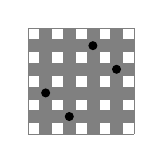
\begin{tikzpicture}[baseline=0.5ex,scale=0.15]
  \tikzstyle{vertex}=[circle,draw=black, fill=black, minimum size=2pt,inner sep=1pt]

  \draw[gray, very thin] (0,0) grid (9,9);
  \fill[gray] (1,0) rectangle (2,9);
  \fill[gray] (3,0) rectangle (4,9);
  \fill[gray] (5,0) rectangle (6,9);
  \fill[gray] (7,0) rectangle (8,9);

  \fill[gray] (0,1) rectangle (9,2);
  \fill[gray] (0,3) rectangle (9,4);
  \fill[gray] (0,5) rectangle (9,6);
  \fill[gray] (0,7) rectangle (9,8);
  
  \node[vertex] (v1) at (1.5, 3.5){};
  \node[vertex] (v2) at (3.5,1.5){};
  \node[vertex] (v3) at (5.5,7.5){};
  \node[vertex] (v4) at (7.5,5.5){};
  \draw (v1) (v2) (v3) (v4);
  \end{tikzpicture}}



\newcommand{\gridabdc}{
  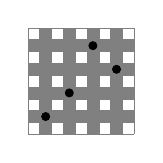
\begin{tikzpicture}[baseline=0.5ex,scale=0.15]
  \tikzstyle{vertex}=[circle,draw=black, fill=black, minimum size=2pt,inner sep=1pt]

  \draw[gray, very thin] (0,0) grid (9,9);
  \fill[gray] (1,0) rectangle (2,9);
  \fill[gray] (3,0) rectangle (4,9);
  \fill[gray] (5,0) rectangle (6,9);
  \fill[gray] (7,0) rectangle (8,9);

  \fill[gray] (0,1) rectangle (9,2);
  \fill[gray] (0,3) rectangle (9,4);
  \fill[gray] (0,5) rectangle (9,6);
  \fill[gray] (0,7) rectangle (9,8);
  
  \node[vertex] (v1) at (1.5, 1.5){};
  \node[vertex] (v2) at (3.5,3.5){};
  \node[vertex] (v3) at (5.5,7.5){};
  \node[vertex] (v4) at (7.5,5.5){};
  \draw (v1) (v2) (v3) (v4);
  \end{tikzpicture}}



\newcommand{\gridbacd}{
  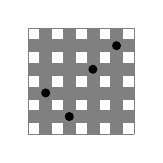
\begin{tikzpicture}[baseline=0.5ex,scale=0.15]
  \tikzstyle{vertex}=[circle,draw=black, fill=black, minimum size=2pt,inner sep=1pt]

  \draw[gray, very thin] (0,0) grid (9,9);
  \fill[gray] (1,0) rectangle (2,9);
  \fill[gray] (3,0) rectangle (4,9);
  \fill[gray] (5,0) rectangle (6,9);
  \fill[gray] (7,0) rectangle (8,9);

  \fill[gray] (0,1) rectangle (9,2);
  \fill[gray] (0,3) rectangle (9,4);
  \fill[gray] (0,5) rectangle (9,6);
  \fill[gray] (0,7) rectangle (9,8);
  
  \node[vertex] (v1) at (1.5, 3.5){};
  \node[vertex] (v2) at (3.5,1.5){};
  \node[vertex] (v3) at (5.5,5.5){};
  \node[vertex] (v4) at (7.5,7.5){};
  \draw (v1) (v2) (v3) (v4);
  \end{tikzpicture}}




%%%%%%%%%%%%%%%%%%%%%%%%%%%%%%%%%%%%%%%%%%%%%%%%%%%%%%%%%%%%%%%%%%%%%%%%%%%%%%%%%%%
% 1-POINT PERMTUATIONS
%%%%%%%%%%%%%%%%%%%%%%%%%%%%%%%%%%%%%%%%%%%%%%%%%%%%%%%%%%%%%%%%%%%%%%%%%%%%%%%%%%%



\newcommand{\atau}{
  \begin{tikzpicture}[baseline=0.5ex,scale=0.15]
  \tikzstyle{vertex}=[circle,draw=black,fill=white, minimum size=2pt,inner sep=1pt]
  \node[vertex] (v1) at (0.5, 0.5){};
  \draw (v1);
  \end{tikzpicture}}

\renewcommand{\a}{
  \begin{tikzpicture}[baseline=0.5ex,scale=0.15]
  \tikzstyle{vertex}=[circle,fill=black, minimum size=2pt,inner sep=1pt]
  \node[vertex] (v1) at (0.5, 0.5){};
  \draw (v1);
  \end{tikzpicture}}


%%%%%%%%%%%%%%%%%%%%%%%%%%%%%%%%%%%%%%%%%%%%%%%%%%%%%%%%%%%%%%%%%%%%%%%%%%%%%%%%%%%
% 2-POINT PERMTUATIONS
%%%%%%%%%%%%%%%%%%%%%%%%%%%%%%%%%%%%%%%%%%%%%%%%%%%%%%%%%%%%%%%%%%%%%%%%%%%%%%%%%%%

\newcommand{\abtau}{
  
\begin{tikzpicture}[baseline=0.5ex,scale=0.15]
  \tikzstyle{vertex}=[circle,draw=black, fill=black, minimum size=2pt,inner sep=1pt]
  \node[vertex] (v1) at (0.5, 0.5){};
  \tikzstyle{vertex}=[circle,draw=black, fill=white, minimum size=2pt,inner sep=1pt]
  \node[vertex] (v2) at (1.5,1.5){};
  %\draw[gray, very thin] (0,0) grid (2,2);
  \draw (v1) (v2);
  \end{tikzpicture}}

\newcommand{\tauab}{
  
\begin{tikzpicture}[baseline=0.5ex,scale=0.15]
  \tikzstyle{vertex}=[circle,draw=black, fill=white, minimum size=2pt,inner sep=1pt]
  \node[vertex] (v1) at (0.5, 0.5){};
  \tikzstyle{vertex}=[circle,draw=black, fill=black, minimum size=2pt,inner sep=1pt]
  \node[vertex] (v2) at (1.5,1.5){};
  %\draw[gray, very thin] (0,0) grid (2,2);
  \draw (v1) (v2);
  \end{tikzpicture}}

\newcommand{\tauba}{
  
\begin{tikzpicture}[baseline=0.5ex,scale=0.15]
  \tikzstyle{vertex}=[circle, draw=black, fill=white, minimum size=2pt,inner sep=1pt]
  \node[vertex] (v1) at (0.5, 1.5){};
  \tikzstyle{vertex}=[circle, draw=black, fill=black, minimum size=2pt,inner sep=1pt]
  \node[vertex] (v2) at (1.5, 0.5){};
  %\draw[gray, very thin] (0,0) grid (2,2);
  \draw (v1) (v2);
  \end{tikzpicture}}

\newcommand{\batau}{
  
\begin{tikzpicture}[baseline=0.5ex,scale=0.15]
  \tikzstyle{vertex}=[circle, draw=black, fill=black, minimum size=2pt,inner sep=1pt]
  \node[vertex] (v1) at (0.5, 1.5){};
  \tikzstyle{vertex}=[circle, draw=black, fill=white, minimum size=2pt,inner sep=1pt]
  \node[vertex] (v2) at (1.5, 0.5){};
  %\draw[gray, very thin] (0,0) grid (2,2);
  \draw (v1) (v2);
  \end{tikzpicture}}


%================ PLAIN ================

\newcommand{\ab}{
  
\begin{tikzpicture}[baseline=0.5ex,scale=0.15]
  \tikzstyle{vertex}=[circle,fill=black, minimum size=2pt,inner sep=1pt]
  \node[vertex] (v1) at (0.5, 0.5){};
  \tikzstyle{vertex}=[circle,fill=black, minimum size=2pt,inner sep=1pt]
  \node[vertex] (v2) at (1.5,1.5){};
  %\draw[gray, very thin] (0,0) grid (2,2);
  \draw (v1) (v2);
  \end{tikzpicture}}

\newcommand{\ba}{
  
\begin{tikzpicture}[baseline=0.5ex,scale=0.15]
  \tikzstyle{vertex}=[circle, fill=black, minimum size=2pt,inner sep=1pt]
  \node[vertex] (v1) at (1.5, 1.5){};
  \tikzstyle{vertex}=[circle, fill=black, minimum size=2pt,inner sep=1pt]
  \node[vertex] (v2) at (0.5, 0.5){};
  %\draw[gray, very thin] (0,0) grid (2,2);
  \draw (v1) (v2);
  \end{tikzpicture}}



%%%%%%%%%%%%%%%%%%%%%%%%%%%%%%%%%%%%%%%%%%%%%%%%%%%%%%%%%%%%%%%%%%%%%%%%%%%%%%%%%%%
% 3-POINT PERMTUATIONS
%%%%%%%%%%%%%%%%%%%%%%%%%%%%%%%%%%%%%%%%%%%%%%%%%%%%%%%%%%%%%%%%%%%%%%%%%%%%%%%%%%%

\newcommand{\tauabc}{
  
\begin{tikzpicture}[baseline=0.5ex,scale=0.15]
  \tikzstyle{vertex}=[circle,draw=black,fill=white, minimum size=2pt,inner sep=1pt]
  \node[vertex] (v1) at (0.5, 0.5){};
  \tikzstyle{vertex}=[circle,fill=black, minimum size=2pt,inner sep=1pt]
  \node[vertex] (v2) at (1.5,1.5){};
  \node[vertex] (v3) at (2.5, 2.5){};
  \draw (v1) (v2) (v3);
  \end{tikzpicture}}

\newcommand{\ataubc}{
  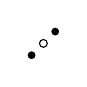
\begin{tikzpicture}[baseline=0.5ex,scale=0.15]
  \tikzstyle{vertex}=[circle,draw=black,fill=white, minimum size=2pt,inner sep=1pt]
  \node[vertex] (v1) at (1.5, 1.5){};
  \tikzstyle{vertex}=[circle,fill=black, minimum size=2pt,inner sep=1pt]
  \node[vertex] (v2) at (0.5,0.5){};
  \node[vertex] (v3) at (2.5, 2.5){};
  \draw (v1) (v2) (v3);
  \end{tikzpicture}}

\newcommand{\acbtau}{
  
\begin{tikzpicture}[baseline=0.5ex,scale=0.15]
  \tikzstyle{vertex}=[circle,draw=black,fill=white, minimum size=2pt,inner sep=1pt]
  \node[vertex] (v1) at (0.5, 0.5){};
  \tikzstyle{vertex}=[circle,fill=black, minimum size=2pt,inner sep=1pt]
  \node[vertex] (v2) at (1.5,2.5){};
  \node[vertex] (v3) at (2.5, 1.5){};
  \draw (v1) (v2) (v3);
  \end{tikzpicture}}


\newcommand{\abc}{
  
\begin{tikzpicture}[baseline=0.5ex,scale=0.15]
  \tikzstyle{vertex}=[circle,fill=black, minimum size=2pt,inner sep=1pt]
  \node[vertex] (v1) at (0.5, 0.5){};
  \node[vertex] (v2) at (1.5,1.5){};
  \node[vertex] (v3) at (2.5, 2.5){};
  \draw (v1) (v2) (v3);
  \end{tikzpicture}}


\newcommand{\acb}{
  
\begin{tikzpicture}[baseline=0.5ex,scale=0.15]
  \tikzstyle{vertex}=[circle,fill=black, minimum size=2pt,inner sep=1pt]
  \node[vertex] (v1) at (0.5, 0.5){};
  \node[vertex] (v2) at (1.5,2.5){};
  \node[vertex] (v3) at (2.5, 1.5){};
  \draw (v1) (v2) (v3);
  \end{tikzpicture}}


\newcommand{\bac}{
  
\begin{tikzpicture}[baseline=0.5ex,scale=0.15]
  \tikzstyle{vertex}=[circle,fill=black, minimum size=2pt,inner sep=1pt]
  \node[vertex] (v2) at (0.5,1.5){};
  \node[vertex] (v1) at (1.5, 0.5){};
  \node[vertex] (v3) at (2.5, 2.5){};
  \draw (v1) (v2) (v3);
  \end{tikzpicture}}

\newcommand{\bca}{
  
\begin{tikzpicture}[baseline=0.5ex,scale=0.15]
  \tikzstyle{vertex}=[circle,fill=black, minimum size=2pt,inner sep=1pt]
  \node[vertex] (v1) at (0.5, 1.5){};
  \node[vertex] (v2) at (1.5,2.5){};
  \node[vertex] (v3) at (2.5, 0.5){};
  \draw (v1) (v2) (v3);
  \end{tikzpicture}}


\newcommand{\cba}{
  
\begin{tikzpicture}[baseline=0.5ex,scale=0.15]
  \tikzstyle{vertex}=[circle,fill=black, minimum size=2pt,inner sep=1pt]
  \node[vertex] (v3) at (0.5, 2.5){};
  \node[vertex] (v2) at (1.5,1.5){};
  \node[vertex] (v1) at (2.5, 0.5){};
  \draw (v1) (v2) (v3);
  \end{tikzpicture}}

\newcommand{\cab}{
  
\begin{tikzpicture}[baseline=0.5ex,scale=0.15]
  \tikzstyle{vertex}=[circle,fill=black, minimum size=2pt,inner sep=1pt]
  \node[vertex] (v1) at (0.5, 2.5){};
  \node[vertex] (v2) at (1.5,0.5){};
  \node[vertex] (v3) at (2.5, 1.5){};
  \draw (v1) (v2) (v3);
  \end{tikzpicture}}

%%%%%%%%%%%%%%%%%%%%%%%%%%%%%%%%%%%%%%%%%%%%%%%%%%%%%%%%%%%%%%%%%%%%%%%%%%%%%%%%%%%
% 4-POINT PERMTUATIONS
%%%%%%%%%%%%%%%%%%%%%%%%%%%%%%%%%%%%%%%%%%%%%%%%%%%%%%%%%%%%%%%%%%%%%%%%%%%%%%%%%%%

\newcommand{\abcd}{
  
\begin{tikzpicture}[baseline=0.6ex,scale=0.1]
  \tikzstyle{vertex}=[circle,fill=black, minimum size=2pt,inner sep=1pt]
  \node[vertex] (v1) at (0.5, 0.5){};
  \node[vertex] (v2) at (1.5, 1.5){};
  \node[vertex] (v3) at (2.5, 2.5){};
  \node[vertex] (v4) at (3.5, 3.5){};
  \draw (v1) (v2) (v3) (v4);
  \end{tikzpicture}}

\newcommand{\bdca}{
  
\begin{tikzpicture}[baseline=0.6ex,scale=0.1]
  \tikzstyle{vertex}=[circle,fill=black, minimum size=2pt,inner sep=1pt]
  \node[vertex] (v1) at (0.5, 1.5){};
  \node[vertex] (v2) at (1.5, 3.5){};
  \node[vertex] (v3) at (2.5, 2.5){};
  \node[vertex] (v4) at (3.5, 0.5){};
  \draw (v1) (v2) (v3) (v4);
  \end{tikzpicture}}

\newcommand{\acdb}{
  
\begin{tikzpicture}[baseline=0.6ex,scale=0.1]
  \tikzstyle{vertex}=[circle,fill=black, minimum size=2pt,inner sep=1pt]
  \node[vertex] (v1) at (0.5, 0.5){};
  \node[vertex] (v2) at (1.5, 2.5){};
  \node[vertex] (v3) at (2.5, 3.5){};
  \node[vertex] (v4) at (3.5, 1.5){};
  \draw (v1) (v2) (v3) (v4);
  \end{tikzpicture}}

%%%%%%%%%%%%%%%%%%%%%%%%%%%%%%%%%%%%%%%%%%%%%%%%%%%%%%%%%%%%%%%%%%%%%%%%%%%%%%%%%%%
% 5-POINT PERMTUATIONS
%%%%%%%%%%%%%%%%%%%%%%%%%%%%%%%%%%%%%%%%%%%%%%%%%%%%%%%%%%%%%%%%%%%%%%%%%%%%%%%%%%%

\newcommand{\bcaoba}{
  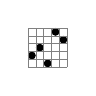
\begin{tikzpicture}[baseline=0.6ex,scale=0.1]
  \tikzstyle{vertex}=[circle,fill=black, minimum size=2pt,inner sep=1pt]
  \node[vertex] (v1) at (0.5, 1.5){};
  \node[vertex] (v2) at (1.5, 2.5){};
  \node[vertex] (v3) at (2.5, 0.5){};
  \node[vertex] (v4) at (3.5, 4.5){};
  \node[vertex] (v5) at (4.5, 3.5){};
  \draw[gray, very thin] (0,0) grid (5,5);
  \draw (v1) (v2) (v3) (v4) (v5);
  \end{tikzpicture}}


\newcommand{\baoaoba}{
  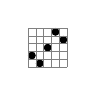
\begin{tikzpicture}[baseline=0.6ex,scale=0.1]
  \tikzstyle{vertex}=[circle,fill=black, minimum size=2pt,inner sep=1pt]
  \node[vertex] (v1) at (0.5, 1.5){};
  \node[vertex] (v2) at (1.5, 0.5){};
  \node[vertex] (v3) at (2.5, 2.5){};
  \node[vertex] (v4) at (3.5, 4.5){};
  \node[vertex] (v5) at (4.5, 3.5){};
  \draw[gray, very thin] (0,0) grid (5,5);
  \draw (v1) (v2) (v3) (v4) (v5);
  \end{tikzpicture}}


\newcommand{\aobamba}{
  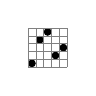
\begin{tikzpicture}[baseline=0.6ex,scale=0.1]
  \tikzstyle{vertex}=[circle,fill=black, minimum size=2pt,inner sep=1pt]
  \node[vertex] (v1) at (0.5, 0.5){};
  \node[vertex] (v2) at (1.5, 3.5){};
  \node[vertex] (v3) at (2.5, 4.5){};
  \node[vertex] (v4) at (3.5, 1.5){};
  \node[vertex] (v5) at (4.5, 2.5){};
  \draw[gray, very thin] (0,0) grid (5,5);
  \draw (v1) (v2) (v3) (v4) (v5);
  \end{tikzpicture}}



%%%%%%%%%%%%%%%%%%%%%%%%%%%%%%%%%%%%%%%%%%%%%%%%%%%%%%%%%%%%%%%%%%%%%%%%%%%%%%%%%%%
% 6-POINT PERMTUATIONS
%%%%%%%%%%%%%%%%%%%%%%%%%%%%%%%%%%%%%%%%%%%%%%%%%%%%%%%%%%%%%%%%%%%%%%%%%%%%%%%%%%%


\newcommand{\bcaocba}{
  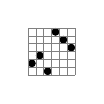
\begin{tikzpicture}[baseline=0.6ex,scale=0.1]
  \tikzstyle{vertex}=[circle,fill=black, minimum size=2pt,inner sep=1pt]
  \node[vertex] (v1) at (0.5, 1.5){};
  \node[vertex] (v2) at (1.5, 2.5){};
  \node[vertex] (v3) at (2.5, 0.5){};
  \node[vertex] (v4) at (3.5, 5.5){};
  \node[vertex] (v5) at (4.5, 4.5){};
  \node[vertex] (v6) at (5.5, 3.5){};
  \draw[gray, very thin] (0,0) grid (6,6);
  \draw (v1) (v2) (v3) (v4) (v5) (v6);
  \end{tikzpicture}}


\newcommand{\bcaobca}{
  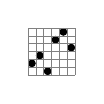
\begin{tikzpicture}[baseline=0.6ex,scale=0.1]
  \tikzstyle{vertex}=[circle,fill=black, minimum size=2pt,inner sep=1pt]
  \node[vertex] (v1) at (0.5, 1.5){};
  \node[vertex] (v2) at (1.5, 2.5){};
  \node[vertex] (v3) at (2.5, 0.5){};
  \node[vertex] (v4) at (3.5, 4.5){};
  \node[vertex] (v5) at (4.5, 5.5){};
  \node[vertex] (v6) at (5.5, 3.5){};
  \draw[gray, very thin] (0,0) grid (6,6);
  \draw (v1) (v2) (v3) (v4) (v5) (v6);
  \end{tikzpicture}}

\newcommand{\bcaocab}{
  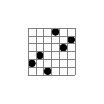
\begin{tikzpicture}[baseline=0.6ex,scale=0.1]
  \tikzstyle{vertex}=[circle,fill=black, minimum size=2pt,inner sep=1pt]
  \node[vertex] (v1) at (0.5, 1.5){};
  \node[vertex] (v2) at (1.5, 2.5){};
  \node[vertex] (v3) at (2.5, 0.5){};
  \node[vertex] (v4) at (3.5, 5.5){};
  \node[vertex] (v5) at (4.5, 3.5){};
  \node[vertex] (v6) at (5.5, 4.5){};
  \draw[gray, very thin] (0,0) grid (6,6);
  \draw (v1) (v2) (v3) (v4) (v5) (v6);
  \end{tikzpicture}}


\newcommand{\baoabmab}{
  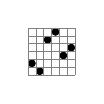
\begin{tikzpicture}[baseline=0.6ex,scale=0.1]
  \tikzstyle{vertex}=[circle,fill=black, minimum size=2pt,inner sep=1pt]
  \node[vertex] (v1) at (0.5, 1.5){};
  \node[vertex] (v2) at (1.5, 0.5){};
  \node[vertex] (v3) at (2.5, 4.5){};
  \node[vertex] (v4) at (3.5, 5.5){};
  \node[vertex] (v5) at (4.5, 2.5){};
  \node[vertex] (v6) at (5.5, 3.5){};
  \draw[gray, very thin] (0,0) grid (6,6);
  \draw (v1) (v2) (v3) (v4) (v5) (v6);
  \end{tikzpicture}}





%%%%%%%%%%%%%%%%%%%%%%%%%%%%%%%%%%%%%%%%%%%%%%%%%%%%%%%%%
%% GRID CLASSES
%%%%%%%%%%%%%%%%%%%%%%%%%%%%%%%%%%%%%%%%%%%%%%%%%%%%%%%%%

\newcommand{\cplusc}[2]{
  \begin{tikzpicture}[baseline=4ex, scale=0.8]
     % \filldraw[black] (0,2) circle (2pt);
      %\draw (-0.3,2.2) node {$\Z$};
      % \draw[-, very thick] (0.2,2.5) -- (0.2,0);
      % \draw[dashed] (0.2,2) -- (2.5,2);
      % \filldraw[black] (2.2,1.6) circle (2pt);
      % \draw (2.6,1.6) node {$\Z$};
      \draw (0,0) rectangle (1,1) node[pos=0.5]{\ensuremath{#1}};
      %\filldraw[black] (0.8,0.3) circle (2pt);
      \draw (1,1) rectangle (2,2) node[pos=0.5]{\ensuremath{#2}};
      % \filldraw[black] (0.8,0.3) circle (2pt);
      %\draw (1.2,0.2) node {$\Z$};
    \end{tikzpicture}}


 \newcommand{\cminusc}[2]{
  \begin{tikzpicture}[baseline=4ex, scale=0.8]
    %\filldraw[black] (0,2) circle (2pt);
      %\draw (-0.3,2.2) node {$\Z$};
      % \draw[-, very thick] (0.2,2.5) -- (0.2,0);
      % \draw[dashed] (0.2,2) -- (2.5,2);
      % \filldraw[black] (2.2,1.6) circle (2pt);
      % \draw (2.6,1.6) node {$\Z$};
      \draw (1,0) rectangle (2,1) node[pos=0.5]{\ensuremath{#1}};
      %\filldraw[black] (0.8,0.3) circle (2pt);
      \draw (0,1) rectangle (1,2) node[pos=0.5]{\ensuremath{#2}};
      % \filldraw[black] (0.8,0.3) circle (2pt);
      %\draw (1.2,0.2) node {$\Z$};
  \end{tikzpicture}}



% -------------- GEOM --------------

\newcommand{\sqr}{
  \hspace{-1.5mm}
  \begin{tikzpicture}[baseline=0.2ex,scale=0.4]
    \filldraw[fill=white!25, draw=black] (0,0) rectangle (1,1);
    %\draw c d1 d2 d3 d4 d5;
  \end{tikzpicture}}


% --------------- PLAIN ----------------

\newcommand{\dts}{
  \hspace{-1.5mm}
  \begin{tikzpicture}[baseline=-0.3ex, scale=0.25]
    \tikzstyle{vertex}=[circle,fill=black, minimum size=2pt,inner sep=1pt]
    \filldraw[fill=white!25, draw=white] (-0.5,-0.5) rectangle (1,1);
    \node (d1) at (-0.2,-0.2){\texttt{.}};
    \node (d2) at (0,0.0){\texttt{.}};
    \node (d3) at (0.2,0.2){\texttt{.}};
    \node (d4) at (0.4,0.4){\texttt{.}};
    \node (d5) at (0.6,0.6){\texttt{.}};
    %\draw c d1 d2 d3 d4 d5;
  \end{tikzpicture}}

\newcommand{\bigdts}{
  \hspace{-1.5mm}
  \begin{tikzpicture}%[baseline=-0.3ex]
    \tikzstyle{vertex}=[circle,fill=black, minimum size=2pt,inner sep=1pt]
    \filldraw[fill=white!25, draw=white] (0,0) rectangle (1,1);
    \draw (0.2,0.2) -- (0.8,0.8);
  \end{tikzpicture}}


\newcommand{\xo}{
%  \hspace{-1.5mm}
  \begin{tikzpicture}[baseline=-0.3ex,scale=0.25]
    \tikzstyle{vertex}=[circle,fill=black, minimum size=2pt,inner sep=1pt]
    \filldraw[fill=white!25, draw=white] (-0.5,-0.5) rectangle (1,1);
    \node[vertex] (d) at (0.2,0.1){};
  \end{tikzpicture}}


\newcommand{\bigxo}{
%  \hspace{-1.5mm}
  \begin{tikzpicture}
    \tikzstyle{vertex}=[circle,fill=black, minimum size=2pt,inner sep=1pt]
    \filldraw[fill=white!25, draw=white] (-0.5,-0.5) rectangle (1,1);
    \filldraw[black](0.25,0.5) circle (1pt);
  \end{tikzpicture}}


\newcommand{\xdts}{
  \hspace{-1.5mm}
  \begin{tikzpicture}[baseline=-0.3ex,scale=0.25]
    \tikzstyle{vertex}=[circle,fill=black, minimum size=2pt,inner sep=1pt]
    \filldraw[fill=white!25, draw=white] (-0.5,-0.5) rectangle (1,1);
    \node (d1) at (-0.3,-0.3){\footnotesize{\texttt{+}}};
    \node (d2) at (0,0.0){\texttt{.}};
    \node (d3) at (0.2,0.2){\texttt{.}};
    \node (d4) at (0.4,0.4){\texttt{.}};
    \node (d5) at (0.6,0.6){\texttt{.}};
    %\draw c d1 d2 d3 d4 d5;
  \end{tikzpicture}}

\newcommand{\bigxdts}{
  \hspace{-1.5mm}
  \begin{tikzpicture}
    \tikzstyle{vertex}=[circle,fill=black, minimum size=2pt,inner sep=1pt]
    \filldraw[fill=white!25, draw=white] (-0.5,-0.5) rectangle (1,1);
    \filldraw[black](0.2,0.2) node{\texttt{+}};
    \draw (0.3,0.3)--(0.8,0.8);
  \end{tikzpicture}}

\newcommand{\xdtso}{
  \hspace{-1.5mm}
  \begin{tikzpicture}[baseline=-0.3ex,scale=0.25]
    \tikzstyle{vertex}=[circle,fill=black, minimum size=2pt,inner sep=1pt]
    \filldraw[fill=white!25, draw=white] (-0.5,-0.5) rectangle (1,1);
    \node (d1) at (-0.3,-0.3){\footnotesize{\texttt{+}}};
    \node (d2) at (0,0.0){\texttt{.}};
    \node (d3) at (0.2,0.2){\texttt{.}};
    \node (d4) at (0.4,0.4){\texttt{.}};
    \node (d5) at (0.7,0.7){\footnotesize{\texttt{o}}};
    %\draw c d1 d2 d3 d4 d5;
  \end{tikzpicture}}

\newcommand{\bigxdtso}{
  \hspace{-1.5mm}
  \begin{tikzpicture}%[baseline=-0.3ex]
    \tikzstyle{vertex}=[circle,fill=black, minimum size=2pt,inner sep=1pt]
    \filldraw[fill=white!25, draw=white] (-0.5,-0.5) rectangle (1,1);
    \filldraw[black](0.2,0.2) node{\texttt{+}};
    \draw (0.3,0.3)--(0.7,0.7);
    \filldraw[black](0.8,0.8) node{\texttt{o}};
  \end{tikzpicture}}

\newcommand{\dtso}{
  \hspace{-1.5mm}
  \begin{tikzpicture}[baseline=-0.3ex,scale=0.25]
    \tikzstyle{vertex}=[circle,fill=black, minimum size=2pt,inner sep=1pt]
    \filldraw[fill=white!25, draw=white] (-0.5,-0.5) rectangle (1,1);
    \node (d1) at (-0.3,-0.3){\texttt{.}};
    \node (d2) at (0,0.0){\texttt{.}};
    \node (d3) at (0.2,0.2){\texttt{.}};
    \node (d4) at (0.4,0.4){\texttt{.}};
    \node (d5) at (0.7,0.7){\footnotesize{\texttt{o}}};
    %\draw c d1 d2 d3 d4 d5;
  \end{tikzpicture}}

\newcommand{\bigdtso}{
  \hspace{-1.5mm}
  \begin{tikzpicture}%[baseline=-0.3ex]
    \tikzstyle{vertex}=[circle,fill=black, minimum size=2pt,inner sep=1pt]
    \filldraw[fill=white!25, draw=white] (-0.5,-0.5) rectangle (1,1);
    \draw (0.2,0.2)--(0.7,0.7);
    \filldraw[black](0.8,0.8) node{\texttt{o}};
  \end{tikzpicture}}

% ------------ RED ---------------------

\newcommand{\dtsred}{
  \hspace{-1.5mm}
  \begin{tikzpicture}[baseline=-0.3ex,scale=0.25]
    \tikzstyle{vertex}=[circle,fill=black, minimum size=2pt,inner sep=1pt]
    \filldraw[fill=red!25, draw=white] (-0.5,-0.5) rectangle (1,1);
    \node (d1) at (-0.2,-0.2){\texttt{.}};
    \node (d2) at (0,0.0){\texttt{.}};
    \node (d3) at (0.2,0.2){\texttt{.}};
    \node (d4) at (0.4,0.4){\texttt{.}};
    \node (d5) at (0.6,0.6){\texttt{.}};
  \end{tikzpicture}}


\newcommand{\xored}{
 % \hspace{-1.5mm}
  \begin{tikzpicture}[baseline=-0.3ex,scale=0.25]
    \tikzstyle{vertex}=[circle,fill=black, minimum size=2pt,inner sep=1pt]
    \filldraw[fill=red!25, draw=white] (-0.5,-0.5) rectangle (1,1);
    \node[vertex] (d) at (0.2,0.1){};
  \end{tikzpicture}}


\newcommand{\xdtsred}{
  \hspace{-1.5mm}
  \begin{tikzpicture}[baseline=-0.3ex,scale=0.25]
    \tikzstyle{vertex}=[circle,fill=black, minimum size=2pt,inner sep=1pt]
    \filldraw[fill=red!25, draw=white] (-0.5,-0.5) rectangle (1,1);
    \node (d1) at (-0.3,-0.3){\footnotesize{\texttt{+}}};
    \node (d2) at (0,0.0){\texttt{.}};
    \node (d3) at (0.2,0.2){\texttt{.}};
    \node (d4) at (0.4,0.4){\texttt{.}};
    \node (d5) at (0.6,0.6){\texttt{.}};
    %\draw c d1 d2 d3 d4 d5;
  \end{tikzpicture}}


\newcommand{\xdtsored}{
  \hspace{-1.5mm}
  \begin{tikzpicture}[baseline=-0.3ex,scale=0.25]
    \tikzstyle{vertex}=[circle,fill=black, minimum size=2pt,inner sep=1pt]
    \filldraw[fill=red!25, draw=white] (-0.5,-0.5) rectangle (1,1);
    \node (d1) at (-0.3,-0.3){\footnotesize{\texttt{+}}};
    \node (d2) at (0,0.0){\texttt{.}};
    \node (d3) at (0.2,0.2){\texttt{.}};
    \node (d4) at (0.4,0.4){\texttt{.}};
    \node (d5) at (0.7,0.7){\footnotesize{\texttt{o}}};
    %\draw c d1 d2 d3 d4 d5;
  \end{tikzpicture}}

\newcommand{\dtsored}{
  \hspace{-1.5mm}
  \begin{tikzpicture}[baseline=-0.3ex,scale=0.25]
    \tikzstyle{vertex}=[circle,fill=black, minimum size=2pt,inner sep=1pt]
    \filldraw[fill=red!25, draw=white] (-0.5,-0.5) rectangle (1,1);
    \node (d1) at (-0.3,-0.3){\texttt{.}};
    \node (d2) at (0,0.0){\texttt{.}};
    \node (d3) at (0.2,0.2){\texttt{.}};
    \node (d4) at (0.4,0.4){\texttt{.}};
    \node (d5) at (0.7,0.7){\footnotesize{\texttt{o}}};
    %\draw c d1 d2 d3 d4 d5;
  \end{tikzpicture}}

% ------------ GREEN ---------------------

\newcommand{\dtsgreen}{
  \hspace{-1.5mm}
  \begin{tikzpicture}[baseline=-0.3ex,scale=0.25]
    \tikzstyle{vertex}=[circle,fill=black, minimum size=2pt,inner sep=1pt]
    \filldraw[fill=green!25, draw=white] (-0.5,-0.5) rectangle (1,1);
    \node (d1) at (-0.2,-0.2){\texttt{.}};
    \node (d2) at (0,0.0){\texttt{.}};
    \node (d3) at (0.2,0.2){\texttt{.}};
    \node (d4) at (0.4,0.4){\texttt{.}};
    \node (d5) at (0.6,0.6){\texttt{.}};
  \end{tikzpicture}}


\newcommand{\xogreen}{
 % \hspace{-1.5mm}
  \begin{tikzpicture}[baseline=-0.3ex,scale=0.25]
    \tikzstyle{vertex}=[circle,fill=black, minimum size=2pt,inner sep=1pt]
    \filldraw[fill=green!25, draw=white] (-0.5,-0.5) rectangle (1,1);
    \node[vertex] (d) at (0.2,0.1){};
  \end{tikzpicture}}


\newcommand{\xdtsgreen}{
  \hspace{-1.5mm}
  \begin{tikzpicture}[baseline=-0.3ex,scale=0.25]
    \tikzstyle{vertex}=[circle,fill=black, minimum size=2pt,inner sep=1pt]
    \filldraw[fill=green!25, draw=white] (-0.5,-0.5) rectangle (1,1);
    \node (d1) at (-0.3,-0.3){\footnotesize{\texttt{+}}};
    \node (d2) at (0,0.0){\texttt{.}};
    \node (d3) at (0.2,0.2){\texttt{.}};
    \node (d4) at (0.4,0.4){\texttt{.}};
    \node (d5) at (0.6,0.6){\texttt{.}};
    %\draw c d1 d2 d3 d4 d5;
  \end{tikzpicture}}


\newcommand{\xdtsogreen}{
  \hspace{-1.5mm}
  \begin{tikzpicture}[baseline=-0.3ex,scale=0.25]
    \tikzstyle{vertex}=[circle,fill=black, minimum size=2pt,inner sep=1pt]
    \filldraw[fill=green!25, draw=white] (-0.5,-0.5) rectangle (1,1);
    \node (d1) at (-0.3,-0.3){\footnotesize{\texttt{+}}};
    \node (d2) at (0,0.0){\texttt{.}};
    \node (d3) at (0.2,0.2){\texttt{.}};
    \node (d4) at (0.4,0.4){\texttt{.}};
    \node (d5) at (0.7,0.7){\footnotesize{\texttt{o}}};
    %\draw c d1 d2 d3 d4 d5;
  \end{tikzpicture}}

\newcommand{\dtsogreen}{
  \hspace{-1.5mm}
  \begin{tikzpicture}[baseline=-0.3ex,scale=0.25]
    \tikzstyle{vertex}=[circle,fill=black, minimum size=2pt,inner sep=1pt]
    \filldraw[fill=green!25, draw=white] (-0.5,-0.5) rectangle (1,1);
    \node (d1) at (-0.3,-0.3){\texttt{.}};
    \node (d2) at (0,0.0){\texttt{.}};
    \node (d3) at (0.2,0.2){\texttt{.}};
    \node (d4) at (0.4,0.4){\texttt{.}};
    \node (d5) at (0.7,0.7){\footnotesize{\texttt{o}}};
    %\draw c d1 d2 d3 d4 d5;
  \end{tikzpicture}}

\begin{titlepage}
    \begin{center}
        \vspace*{1cm}
        
        \Huge
        \textbf{PACKING AND COUNTING PERMUTATIONS}
        
        \vspace{1.5cm}
        
        \textbf{Jakub Slia\v{c}an}
        
        \vfill
        
        \Large a thesis submitted to The Open University\\
        for the degree of Doctor of Philosophy in Mathematics
        
        \vspace{0.8cm}
        
        \includegraphics[width=0.4\textwidth]{figs/oulogo.jpg}
        
        \vspace{0.8cm}

        \Large
        February 2017
        
    \end{center}
\end{titlepage}
\afterpage{\null\newpage}

\setcounter{secnumdepth}{-3}% default for "report" is 2
\chapter{Abstract}
A permutation class is a set of permutations closed under taking subpermutations. We study two aspects of permutation classes: enumeration and packing.

Our work on enumeration consists of two campaigns. First, we enumerate all juxtaposition classes of the form ``$\Av(abc)$ next to $\Av(xy)$'', where $abc$ and $xy$ are permutations of lengths three and two, respectively. We represent elements from such a juxtaposition class by Dyck paths decorated with sequences of points. Context-free grammars are then used to enumerate these decorated Dyck paths. Second, we classify as algebraic the generating functions of $1\times m$ permutation grid classes where one cell is context-free and the remaining cells are monotone. We rely on properties of combinatorial specifications of context-free classes and use operators to express juxtapositions. Repeated application of operators resolves cases for $m>2$. We provide examples to re-prove known results and give new ones. Our methods are algorithmic and could be implemented on a PC.

Our work on packing consolidates current knowledge about packing densities of 4-point permutations. We also improve the lower bounds for the packing densities of 1324 and 1342 and provide rigorous upper bounds for the packing densities of 1324, 1342, and 2413. All our bounds are within $10^{-4}$ of the true packing densities. Together with the known bounds, we have a fairly complete picture of 4-point packing densities. Additionally, we obtain several bounds (lower and upper) for permutations of length at least five. Our main tool for the upper bounds is the framework of flag algebras introduced by Razborov in 2007. We also present Permpack --- a flag algebra package for permutations. 
\afterpage{\null\newpage}

\chapter{Acknowledgements}
I would like to thank my supervisor Robert Brignall for finding nice balance between guidance and freedom. I especially valued the opportunity to pursue side projects with little or no relationship to my thesis without the pressure of producing measurable results. It made mathematics more enjoyable. Thank you.

My acknowledgements go to the Department of Mathematics and Statistics at The Open University for funding my PhD and providing support in various forms throughout the past three years.

Special thanks go to my office mates who tolerated my smelly running clothes as well as my constant chewing in our office: Grahame Erskine, Michael Ewetola, Jay Fraser, and Olivia Jeans. I am particularly grateful to David Bevan for his welcome when I first came to the department, for maths conversations and help. Thanks also go to Lax Chan, Argyris Christodoulou, Ioannis Dourekas, Vasso Evdoridou, Matthew Jacques, Robert Lewis, Alison Maidment, David Marchant, Maha Moustafa, David Mart\'{i}-Pete, Tony Royle, Margaret Stanier, Brigitte Stenhouse, and James Tuite.

Additionally, I would like to thank my co-authors, collaborators, and influences outside of my department: Dan Kr\'a\v{l}, Oleg Pikhurko, Jozef Skokan, Kostas Tyros, Walter Stromquist, and Michael Albert.

Thanks also go to my parents and Veronika for being supportive throughout.

Lastly, I thank Fiona who helps me stay mathematically curious.
\afterpage{\null\newpage}

\chapter{Declarations}
There are five chapters in this thesis.
\begin{enumerate}
\item Chapter~\ref{chap:general_intro} consists of a general exposition of the area of permutation patterns and the two viewpoints of the area that we take in this thesis: enumeration and packing. Most of the text in this chapter follows parts of the comprehensive exposition in Bevan's thesis~\cite{bevan2015thesis}.
\item Chapter~\ref{chap:catalanjuxt} consists of joint work with Robert Brignall. The corresponding paper~\cite{brignallsliacanjuxt} is published in \emph{Electronic Journal of Combinatorics}. We use PermLab~\cite{albertpermlab}, Mathematica~\cite{mathematica} and Sage~\cite{sagemath} for computations.
\item Chapter~\ref{chap:iterjuxt} consists of joint work with Robert Brignall. We use PermLab~\cite{albertpermlab} and Mathematica~\cite{mathematica} for our computations.
\item Chapter~\ref{chap:packsmall} consists of joint work with Walter Stromquist. The corresponding paper~\cite{sliacanstromquistpacking} is published in \emph{Discrete Mathematics and Theoretical Computer Science} in \emph{Permutation Patterns 2016} special issue. We make use of: Flagmatic package~\cite{flagmatic}, Mathematica~\cite{mathematica}, Sage~\cite{sagemath}, and Permpack~\cite{permpack}.
\item Chapter~\ref{chap:permpack} consists of a description of Permpack that the author wrote for the work in Chapter~\ref{chap:packsmall}. It was written to resemble Flagmatic to make it easier to use alongside Flagmatic. No Flagmatic code was used, nor were any algorithms taken into Permpack. Permpack is a Sage~\cite{sagemath} package.
\end{enumerate}
None of the results appear in any other thesis and all co-authors have agreed with inclusion of joint work in this thesis.
\afterpage{\null\newpage}


\setlength{\parskip}{0em}
\setcounter{secnumdepth}{3}
\tableofcontents
\setlength{\parskip}{1em}
\chapter{General Introduction}
\label{chap:general_intro}
\begin{center}
\emph{Enumerating permutations is sometimes hard and usually tedious. Packing permutations is often hard and always tedious.}
\end{center}
\begin{flushright}
  \vspace{-15pt}
  --- folklore
  \vspace{20pt}
\end{flushright}



This entire thesis is concerned with only one kind of object --- \emph{permutations}. We treat permutations as patterns or words that use every letter in the alphabet exactly once, the alphabet being $[n] = \{1,\ldots,n\}$. In fact, we study permutation classes rather than permutations themselves. These are collections of permutations closed under taking subpermutations. There are several natural approaches to studying permutation classes. Let $\C$ be a permutation class. Then one can enquire about the properties of a what a typical object from $\C$ ``looks'' like? Alternatively, one could be interested in how many permutations of each length are there in $\C$? Yet another different approach would be to ask questions such as what is the maximum number of inversions that a permutation in $\C$ can have? While all three are interesting directions of study, we focus on questions of the second and third kinds only.

The enumerative approach to permutation classes has been quite dominant in the permutation patterns community. There are several works that survey this area chronologically and systematically. We point to the chapter \emph{Permutation Classes} by Vatter~\cite{vatterhandbook} in the Handbook of Enumerative Combinatorics. For further book material, refer to the references therein. On the other hand, additional surveys of the field can be found in the conference proceedings of Permutation Patterns 2007~\cite{lintonruskucvatter}. The contributions relevant to this thesis are \emph{A survey of simple permutations} by Brignall~\cite{brignallsimple}, \emph{An introduction to structural methods in permutation patterns} by Albert~\cite{albertstructural}, and parts of \emph{Some general results in combinatorial enumeration} by Klazar~\cite{klazargeneral}. Another relevant survey is \emph{Some open problems on permutation patterns} by Steingrimsson~\cite{einar2012openproblems}. The general background of enumerative combinatorics from the perspective of generating functions via the \emph{symbolic method} is best treated in \emph{Analytic Combinatorics} by Flajolet and Sedgewick~\cite{analcomb}.

Permutation packing has been less prevalent among research topics in the area of permutation patterns. The single best survey article, containing new (at that time) results, is \emph{On packing densities of permutations} by Albert, Atkinson, Handley, Holton, and Stromquist~\cite{albert2002packing}. Although there have been significant advances in permutation packing since 2002, there have not been many of them, e.g.~Barton~\cite{barton2004packing} or Presutti and Stromquist~\cite{presutti2010packing}. Hence the article is still relevant in 2018.

\section{Concepts and definitions}
We now proceed to define key concepts needed throughout the thesis. We postpone the particular definitions needed in individual chapters to those chapters. A \emph{pattern} of length $k$, where $k \leq n$, is a $k$-tuple of distinct integers from $[n] :=\{1,\ldots,n\}$. A pattern of length $n$ is called a \emph{permutation}. We write tuples as strings: 1324 stands for $(1,3,2,4)$. Two patterns $\pi$ and $\sigma$ of length $k$ are \emph{identical}, if $\pi[i] = \sigma[i]$ for all $i \in [k]$. They are \emph{order-isomorphic} if for all pairs of indices $i,j$, it holds that $\pi[i] <\pi[j]$ if and only if $\sigma[i] < \sigma[j]$. For a set $I = \{i_1,\ldots,i_m\}$ of $m$ indices from $[n]$, the \emph{sub-pattern} $\pi[I]$ is the $m$-tuple $\pi[i_1]\pi[i_2]\cdots \pi[i_m]$. By overloading the notation slightly, we also use $\pi[I]$ to refer to the \emph{subpermutation} of length $m$ which is order-isomorphic to the sub-pattern $\pi[I]$. Finally, we do not distinguish between different representations of the same permutation. For example, 2413 and its plot on the grid in Figure~\ref{fig:im2413} will be referred to as 2413 interchangeably. Let $\F$ be a set of \emph{forbidden} permutations. We say that permutation $\pi$ is \emph{$\F$-free} if no $\phi\in\F$ is a subpermutation of $\pi$. Such $\pi$ is also said to \emph{avoid} $\F$ or be \emph{admissible}. 


\begin{figure}[ht]
  \begin{center}
    \begin{subfigure}[b]{0.3\textwidth}
      \centering
      \begin{tikzpicture}[scale=0.5]
        \draw[gray] (0,0) grid (4,4);
        \filldraw[black] (0.5,0.5) circle (8pt);
        \filldraw[black] (1.5,1.5) circle (8pt);
        \filldraw[black] (2.5,2.5) circle (8pt);
        \filldraw[black] (3.5,3.5) circle (8pt);
      \end{tikzpicture}
      \caption{1234}
    \end{subfigure}
    \begin{subfigure}[b]{0.3\textwidth}
      \centering
      \begin{tikzpicture}[scale=0.5]
        \draw[gray] (0,0) grid (4,4);
        \filldraw[black] (0.5,0.5) circle (8pt);
        \filldraw[black] (1.5,1.5) circle (8pt);
        \filldraw[black] (2.5,3.5) circle (8pt);
        \filldraw[black] (3.5,2.5) circle (8pt);
      \end{tikzpicture}
      \caption{1243}
    \end{subfigure}
    \begin{subfigure}[b]{0.3\textwidth}
      \centering
      \begin{tikzpicture}[scale=0.5]
        \draw[gray] (0,0) grid (4,4);
        \filldraw[black] (0.5,1.5) circle (8pt);
        \filldraw[black] (1.5,3.5) circle (8pt);
        \filldraw[black] (2.5,0.5) circle (8pt);
        \filldraw[black] (3.5,2.5) circle (8pt);
      \end{tikzpicture}
      \caption{2413}
    \end{subfigure}

  \end{center}
  \caption{Pictorial representations of selected permutations.}
  \label{fig:im2413}
\end{figure}
    
\subsection{Special permutations}

An \emph{interval} refers to a set of integers appearing contiguously in a permutation, e.g. $3645$ is an interval in $213645$. A permutation $\pi$ is \emph{simple} if it does not contain any non-trivial intervals. For instance, $2413$ is simple while $1243$ is not (both $12$ and $43$ are intervals). We call $\pi$ an \emph{inflation} of $\sigma$ if it can be obtained from $\sigma$ by substituting points of $\sigma$ for permutations. We denote $\pi$ as an inflation of $\sigma$ by $\pi = \sigma[\alpha_1,\ldots,\alpha_{|\sigma|}]$, where $\alpha_1,\ldots,\alpha_{|\sigma|}$ are permutations that inflate $\sigma$ into $\pi$. Consider the example of $1243$ as an inflation of $12$, so $1243 = 12[12,21]$. In this case, it is also an inflation of $12$ by $1$ and $132$ as in $1243=12[1,132]$. There is a fundamental result by Albert and Atkinson~\cite{albertatkinsonrestricted} which says that if $\sigma$ is of length at least three and simple, then for any $\pi$ which is an inflation of $\sigma$ there is always a unique way to inflate $\sigma$ into $\pi$. Hence, $12$ and $21$ are special. 

A \emph{decreasing (increasing) permutation} of length $k$ is $k\ldots321$, respectively $123\ldots k$. A permutation $\pi$ is \emph{layered}, if it is an increasing sequence of decreasing permutations. To be exact, a layered permutation $\pi$ is a concatenation of smaller permutations $\pi= \pi_1\pi_2\ldots\pi_\ell$ such that for all $1 \leq i \leq \ell$, $\pi_i$ is a decreasing sequence of consecutive integers satisfying the following: if $x \in \pi_i$ and $y \in \pi_j$ with $i<j$, then $x<y$. For instance, 321465987 can be partitioned as $321|4|65|987$, so it is layered. On the other hand, 2413 is not layered. This brings us to the notion of sum and skew-sum of permutations. Let $\pi_1$ and $\pi_2$ be permutations of lengths $k$ and $\ell$. We say that $\pi$ is a \emph{sum of $\pi_1$ and $\pi_2$}, denoted by $\pi = \pi_1\oplus\pi_2$, if $\pi$ consists of two intervals $\pi[1]\cdots\pi[k]$ and $\pi[k+1]\cdots\pi[\ell]$ such that $\pi[1]\cdots\pi[k]$ is order-isomorphic to $\pi_1$, $\pi[k+1]\cdots\pi[\ell]$ is order-isomorphic to $\pi_2$, and $\pi[i] < \pi[j]$ for all $i\leq k$ and $j>k$. Similarly, $\pi$ is a \emph{skew-sum of $\pi_1$ and $\pi_2$}, denoted by $\pi = \pi_1\ominus \pi_2$, if $\pi$ consists of the two intervals as above, except this time we require that $\pi[i] > \pi[j]$ for all $i\leq k$ and $j > k$. A permutation is called \emph{sum-indecomposable} if it cannot be expressed as a sum of two non-empty permutations. Analogously, \emph{skew-indecomposable} permutations cannot be expressed as skew sums of non-empty permutations. With this new notation in place, a layered permuation with $k$ layers is $\pi = \pi_1\oplus\cdots\oplus \pi_k$ such that all $\pi_i$ are decreasing permutations. A permutation is called \emph{separable}, if it can be obtained from single points by repeated application of sum and skew-sum. For instance, $42315=(1\ominus (1\oplus 1)\ominus 1)\oplus 1$ is separable, but $2413$ is not.

\subsection{Permutation classes}
A \emph{permutation class} $\C$ is a set of permutations which is closed under taking subpermutations, i.e. if $\pi$ is in $\C$ and $\sigma \subseteq \pi$, then $\sigma$ is also in $\C$. Given that the subpermutation relation is a partial order on a permutation class $\C$, there is a minimal set of forbidden permutations called the \emph{basis} $\B$ of $\C$. We also write $\C = \Av(\B)$ to make explicit the fact that $\C$ is the set of avoiders of $\B$. For example, the class $\Av(231,312)$ is the class of layered permutations. Similarly, $\Av(2413, 3142)$ is the class of separable permutations. The subset of a class $\C$ containing only permutations of length $n$ is referred to by $\C_n$. Hence, $\C = \bigcup_{n\geq0}\C_n$. We use $|\C_n|$ to denote the number of elements of length $n$ in $\C$. 

To enumerate a permutation class $\C$ means to provide a sequence $(a_n)_{n\geq 0}$ such that $a_n = |\C_n|$. Given that $(a_n)_n$ has infinitely many terms, we need a clever data structure to store it in finite memory. A \emph{generating function} $C(z)$ of $\C$ is a formal power series $C(z) = \sum_{n\geq 0}a_nz^n$ with the coefficient of $z^n$ being the $n$-th term of the sequence. Ideally we would know the closed form of $C(z)$, e.g. the closed form of $C(z) = \sum_{n\geq 0}z^n = 1/(1-z)$. A rational generating function is one whose closed form is a ratio of two polynomials. An algebraic generating function $f = f(z)$ is a root of a polynomial equation in $f$ and $z$. As a shortcut, when we say that a generating function enumerating $\C$ is rational/algebraic/etc., we mean that the closed form of the formal power series storing the counting sequence which enumerates $\C$ is rational/algebraic/etc.

All work in this thesis is on enumeration of permutation (grid) classes. Whenever we obtain a generating function and a counting sequence, we refer to the result as an ``exact enumeration''. On the other hand, if we can only comment on the quality of the generating function yet we did not find one explicitly, we do not use the term ``exact''. This constitutes a slight deviation from the customary usage of the term ``exact enumeration''. We do not use ``exact'' to create contrast against ``asymptotic''. Mentioning it here hopefully prevents confusion later on.


It may not always be possible to find the generating function for a class. One cruder way of ``enumerating'' a permutation class is \emph{asymptotically}, by determining its growth rate. The \emph{growth rate} of a class $\C$ is denoted by $\gr{\C}$ and is defined as below provided that the limit exists.
$$\gr{\C} = \lim_{n\to\infty}\sqrt[n]{|\C_n|}$$
Naturally, if the above limit does not exist despite being conjectured to always exist, we speak about an \emph{upper growth rate} of $\C$ defined as $\lim\sup_{n\to\infty}\sqrt[n]{|\C_n|}$ and a \emph{lower growth rate} of $\C$ defined as $\lim\inf_{n\to\infty}\sqrt[n]{|\C_n|}$. Conveniently, by proving F\"{u}redi-Hajnal conjecture, Marcus and Tardos~\cite{marcus04growthrate} also proved Stanley-Wilf conjecture that the upper growth rate is finite for all proper permutation classes. Together with Arratia's observation in~\cite{arratia1999}, this implies that all permutation classes with basis of size one --- also called \emph{principal} classes --- have finite growth rates. Interestingly, there were conjectures about the growth rates of principal classes and all were refuted by this point in time. First Arratia~\cite{arratia1999} conjectured that for every permutation $\sigma$, $\gr{\Av(\sigma)} \leq (k-1)^2$. However, in 2006 Albert, Elder, Rechnitzer, Westcott, and Zabrocki~\cite{albert2006wilf} disproved this by showing that $\gr{\Av(1324)} > 9.47 > (4-1)^2$. B\'ona first suggested in~\cite{bona2005wilf} that layered permutations may be the easiest to avoid, i.e. their principal avoider classes tend to have highest growth rates, an impression strengthened by the result of Albert et al.~\cite{albert2006wilf}. However, in 2013 Fox~\cite{fox2013wilf} confirmed what we knew already: that we do not understand the growth rates of permutation classes very well. His result states that almost all patterns $\sigma$ of length $k$ have growth rates of a completely different order than we thought: $\gr{\Av(\sigma)} = 2^{\Omega(k)}$. Although this was tangential to the core topic of the thesis, it shows that permutation patterns form an exciting area to study.




\part{Enumeration} %%%%%%%%%%%%%%%%%%%%%%%%%%%%%%%%%%%%%%%%%%%%%%%%%%%%%
\label{part:enumeration}

\chapter{Introduction to Enumeration}
\label{chap:enumintro}

This chapter contains results on enumeration of permutation grid classes. They are useful given that one of the approaches to enumerating permutation classes is through permutation \emph{grid classes}. These are permutation classes themselves but offer additional insight into structure of the permutations in them. For instance, if a permutation $\sigma$ can be split by a vertical line into a left part and a right part so that the left part (as a subpermutation of $\sigma$) avoids 21 and the right part avoids 12, then $\sigma$ belongs to $\C = \Av(21|12)$, a $1\times 2$ grid class with the left cell being $\Av(21)$ and the right cell being $\Av(12)$. All permutations in $\C$ can be split this way, and all permutations that admit such gridding belong to $\C$. \\

The grid class that we just described, in our notation $\Av(21)|\Av(12)$, was enumerated by Atkinson~\cite{atkinson1998incrdecr}. In~\cite{atkinson1997restricted}, Atkinson used grid classes to enumerate other classes such as $\Av(132,4321)$, $\Av(321,2134)$, and $\Av(321,1324)$ (Bevan calls these ``skinny grid classes'' in his thesis~\cite{bevan2015thesis}). In recent years, grid classes were critical to enumeration of two-by-four classes with two basis elements of length four. See Pantone~\cite{pantone2by4} for enumeration of $\Av(3124,4312)$. Albert, Atkinson, and Brignall used grid classes to enumerate $\Av(2143,4231)$ in~\cite{albert2011enumeration} and three other two-by-four classes in~\cite{albert2012gridclasses}. Albert, Atkinson, and Vatter~\cite{albert2012inflations} use a special kind of grid classes to enumerate three specific permutation classes. Another paper making use of grid classes to enumerate $\Av(4231, 35142, 42513, 351624)$ is by Albert and Brignall~\cite{albert2014schubert}. We also mention Bevan's enumeration of $\Av(4213,2143)$ in~\cite{bevan-new} which utilizes permutation grid classes. 

Recall that a growth rate of a permutation class $\C$ is defined as $\lim_{n}\sqrt[n]{|\C_n|} = \lim\inf_{n}\sqrt[n]{|\C_n|}=\lim\sup_{n}\sqrt[n]{|\C_n|}$ if it exists. Grid classes have been central to Vatter's proof~\cite{vatter11small} of the fact that there are only countably many growth rates of permutation classes below $\xi \approx 2.30522$ while there are uncountably many growth rates arbitrarily close to $\xi$. Two follow-up papers of Vatter~\cite{vattercountableuncountable}, and Pantone and Vatter~\cite{pantonevatter16categorize} make use of grid classes as well.

Apart from enumerating permutation classes, several other applications of grid classes exist, among them~\cite{albert2011enumeration} and~\cite{bevan-new}. We give further examples, with accompanying commentaries, in the next paragraph. For a comprehensive introduction to grid classes and their further uses, see Bevan's PhD thesis~\cite{bevan2015thesis}, Sections 2 and 6 in Part I, as well as parts of the general introduction in Section 1 of Part I.

Because of their more general applicability, the study of grid classes in their own right has emerged in a few directions. For instance, it is conjectured that all monotone grid classes are finitely based, but this is only known for a few special cases, most notably those whose row-column graph is acyclic~\cite{aabrv2013}, and a few other special cases (see~\cite{albert-brignall-2times2, atkinson1997restricted, waton, bevan2015thesis}). In another direction, the role of grid classes with respect to partial well-ordering has been explored in e.g.~\cite{brignall2012pwo, murphy2003pwo, vatter2011pwo}. Finally, while the asymptotic enumeration of monotone grid classes was answered completely by Bevan~\cite{bevan15growth-rates}, exact enumeration is harder, primarily due to the difficulty of handling multiple griddings: that is, enumerating `griddable' objects rather than `gridded' ones. One general result here is that all geometric grid classes have rational generating functions~\cite{aabrv2013}, but the move from `gridded' to `griddable' is nonconstructive, instead relying on properties of regular languages.

Since grid classes are often used on the way to enumerating other permutation classes, it would be convenient to be able to enumerate grid classes. Ideally, we would have exact enumerations of classes of the form shown in Figure~\ref{fig:genericgridclass} --- the most generic form of grid classes. For the current level of discussion, Figure~\ref{fig:genericgridclass} also suffices as a definition of a grid class (a grid of permutation classes).

\begin{figure}[ht!]
\begin{center}
\begin{tikzpicture}[scale=0.8]
  \draw[gray, very thin] (0,0) grid (4,4);
  \draw[gray, very thin] (0,0) -- (0,-0.5);
  \draw[gray, very thin] (1,0) -- (1,-0.5);
  \draw[gray, very thin] (2,0) -- (2,-0.5);
  \draw[gray, very thin] (3,0) -- (3,-0.5);
  \draw[gray, very thin] (4,0) -- (4,-0.5);

  \draw[gray, very thin] (4,4) -- (4.5,4);
  \draw[gray, very thin] (4,3) -- (4.5,3);
  \draw[gray, very thin] (4,2) -- (4.5,2);
  \draw[gray, very thin] (4,1) -- (4.5,1);
  \draw[gray, very thin] (4,0) -- (4.5,0);

  \draw[gray, very thin] (6.5,4) -- (7,4);
  \draw[gray, very thin] (6.5,3) -- (7,3);
  \draw[gray, very thin] (6.5,2) -- (7,2);
  \draw[gray, very thin] (6.5,1) -- (7,1);
  \draw[gray, very thin] (6.5,0) -- (7,0);
  \draw[gray, very thin] (7,4) -- (7,-0.5);

  \draw[gray, very thin] (0,-2.5) -- (0,-3);
  \draw[gray, very thin] (1,-2.5) -- (1,-3);
  \draw[gray, very thin] (2,-2.5) -- (2,-3);
  \draw[gray, very thin] (3,-2.5) -- (3,-3);
  \draw[gray, very thin] (4,-2.5) -- (4,-3);
  \draw[gray, very thin] (0,-3) -- (4.5,-3);

  \draw[gray, very thin] (7,-3) -- (6.5,-3);
  \draw[gray, very thin] (7,-3) -- (7,-2.5);
  \node at (0.5, 3.5){$\C_{11}$};
  \node at (1.5, 3.5){$\C_{12}$};
  \node at (2.5, 3.5){$\C_{13}$};


  \node at (0.5, 2.5){$\C_{21}$};
  \node at (1.5, 2.5){$\C_{22}$};
  \node at (2.5, 2.5){$\C_{23}$};


  \node at (0.5, 1.5){$\C_{31}$};
  \node at (1.5, 1.5){$\C_{32}$};
  \node at (2.5, 1.5){$\C_{33}$};

  \node at (2.5, -1.5){$\vdots$};
  \node at (5.5, -1.5){$\ddots$};
  \node at (5.5, 1.5){$\ldots$};

  \node at (0.5, -2.5){$\C_{n1}$};
  \node at (1.5, -2.5){$\C_{n2}$};
  \node at (2.5, -2.5){$\C_{n3}$};
  \node at (6.5, 3.5){$\C_{1m}$};
  \node at (6.5, 2.5){$\C_{2m}$};
  \node at (6.5, 1.5){$\C_{3m}$};
  \node at (6.5, -2.5){$\C_{nm}$};
\end{tikzpicture}
\end{center}
\caption{A generic format of a generalised grid class, where $\C_{ij}$ are arbitrary but fixed permutation classes.}
\label{fig:genericgridclass}
\end{figure}

The current state of affairs is much more grim. We cannot even enumerate grid classes of the form shown in Figure~\ref{fig:oneC} or in Figure~\ref{fig:allM}. However, there are several important results in this direction. For instance, due to Bevan~\cite{bevan15growth-rates} we at least know the growth rates of monotone grid classes (where every cell is monotone, like Figure~\ref{fig:allM}). The growth rates are equal to the square of the spectral radius of a certain associated row-column graph.

\begin{figure}[ht!]
  \centering
  \begin{subfigure}{0.45\textwidth}
    \centering
    \begin{tikzpicture}[scale=0.6]
  \draw[gray, very thin] (0,0) grid (4,4);
  \draw[gray, very thin] (0,0) -- (0,-0.5);
  \draw[gray, very thin] (1,0) -- (1,-0.5);
  \draw[gray, very thin] (2,0) -- (2,-0.5);
  \draw[gray, very thin] (3,0) -- (3,-0.5);
  \draw[gray, very thin] (4,0) -- (4,-0.5);

  \draw[gray, very thin] (4,4) -- (4.5,4);
  \draw[gray, very thin] (4,3) -- (4.5,3);
  \draw[gray, very thin] (4,2) -- (4.5,2);
  \draw[gray, very thin] (4,1) -- (4.5,1);
  \draw[gray, very thin] (4,0) -- (4.5,0);

  \draw[gray, very thin] (6.5,4) -- (7,4);
  \draw[gray, very thin] (6.5,3) -- (7,3);
  \draw[gray, very thin] (6.5,2) -- (7,2);
  \draw[gray, very thin] (6.5,1) -- (7,1);
  \draw[gray, very thin] (6.5,0) -- (7,0);
  \draw[gray, very thin] (7,4) -- (7,-0.5);

  \draw[gray, very thin] (0,-2.5) -- (0,-3);
  \draw[gray, very thin] (1,-2.5) -- (1,-3);
  \draw[gray, very thin] (2,-2.5) -- (2,-3);
  \draw[gray, very thin] (3,-2.5) -- (3,-3);
  \draw[gray, very thin] (4,-2.5) -- (4,-3);
  \draw[gray, very thin] (0,-3) -- (4.5,-3);

  \draw[gray, very thin] (7,-3) -- (6.5,-3);
  \draw[gray, very thin] (7,-3) -- (7,-2.5);
  \node at (0.5, 3.5){$\M$};
  \node at (1.5, 3.5){$\M$};
  \node at (2.5, 3.5){$\M$};
  \node at (3.5, 3.5){$\M$};


  \node at (0.5, 2.5){$\M$};
  \node at (1.5, 2.5){$\M$};
  \node at (2.5, 2.5){\textcolor{red}{$\C$}};
  \node at (3.5, 2.5){$\M$};


  \node at (0.5, 1.5){$\M$};
  \node at (1.5, 1.5){$\M$};
  \node at (2.5, 1.5){$\M$};
  \node at (3.5, 1.5){$\M$};

  \node at (2.5, -1.5){$\vdots$};
  \node at (5.5, -1.5){$\ddots$};
  \node at (5.5, 1.5){$\ldots$};

  \node at (0.5, -2.5){$\M$};
  \node at (1.5, -2.5){$\M$};
  \node at (2.5, -2.5){$\M$};
  \node at (6.5, 3.5){$\M$};
  \node at (6.5, 2.5){$\M$};
  \node at (6.5, 1.5){$\M$};
  \node at (6.5, -2.5){$\M$};
\end{tikzpicture}
\caption{All cells are monotone except for $\C$, which is a more complex class.}
\label{fig:oneC}
\end{subfigure}\hfill
\begin{subfigure}{0.45\textwidth}
  \centering
  \begin{tikzpicture}[scale=0.6]
  \draw[gray, very thin] (0,0) grid (4,4);
  \draw[gray, very thin] (0,0) -- (0,-0.5);
  \draw[gray, very thin] (1,0) -- (1,-0.5);
  \draw[gray, very thin] (2,0) -- (2,-0.5);
  \draw[gray, very thin] (3,0) -- (3,-0.5);
  \draw[gray, very thin] (4,0) -- (4,-0.5);

  \draw[gray, very thin] (4,4) -- (4.5,4);
  \draw[gray, very thin] (4,3) -- (4.5,3);
  \draw[gray, very thin] (4,2) -- (4.5,2);
  \draw[gray, very thin] (4,1) -- (4.5,1);
  \draw[gray, very thin] (4,0) -- (4.5,0);

  \draw[gray, very thin] (6.5,4) -- (7,4);
  \draw[gray, very thin] (6.5,3) -- (7,3);
  \draw[gray, very thin] (6.5,2) -- (7,2);
  \draw[gray, very thin] (6.5,1) -- (7,1);
  \draw[gray, very thin] (6.5,0) -- (7,0);
  \draw[gray, very thin] (7,4) -- (7,-0.5);

  \draw[gray, very thin] (0,-2.5) -- (0,-3);
  \draw[gray, very thin] (1,-2.5) -- (1,-3);
  \draw[gray, very thin] (2,-2.5) -- (2,-3);
  \draw[gray, very thin] (3,-2.5) -- (3,-3);
  \draw[gray, very thin] (4,-2.5) -- (4,-3);
  \draw[gray, very thin] (0,-3) -- (4.5,-3);

  \draw[gray, very thin] (7,-3) -- (6.5,-3);
  \draw[gray, very thin] (7,-3) -- (7,-2.5);
  \node at (0.5, 3.5){$\M$};
  \node at (1.5, 3.5){$\M$};
  \node at (2.5, 3.5){$\M$};
  \node at (3.5, 3.5){$\M$};


  \node at (0.5, 2.5){$\M$};
  \node at (1.5, 2.5){$\M$};
  \node at (2.5, 2.5){$\M$};
  \node at (3.5, 2.5){$\M$};


  \node at (0.5, 1.5){$\M$};
  \node at (1.5, 1.5){$\M$};
  \node at (2.5, 1.5){$\M$};
  \node at (3.5, 1.5){$\M$};

  \node at (2.5, -1.5){$\vdots$};
  \node at (5.5, -1.5){$\ddots$};
  \node at (5.5, 1.5){$\ldots$};

  \node at (0.5, -2.5){$\M$};
  \node at (1.5, -2.5){$\M$};
  \node at (2.5, -2.5){$\M$};
  \node at (6.5, 3.5){$\M$};
  \node at (6.5, 2.5){$\M$};
  \node at (6.5, 1.5){$\M$};
  \node at (6.5, -2.5){$\M$};
\end{tikzpicture}
\caption{All cells are monotone (increasing or decreasing).}
\label{fig:allM}
\end{subfigure}
\caption{We cannot enumerate either of the two grid classes in~\ref{fig:oneC} and~\ref{fig:allM}.}
\label{fig:wecantdo}
\end{figure}

Approaching the topic from another angle, Albert, Atkinson, Bouvel, Ru\v{s}kuc and Vatter~\cite{aabrv2013} proved that geometric monotone grid classes are enumerated by \emph{rational} generating functions. Notice that this result is different from the exact enumeration type of results. And that along two dimensions. First, the authors do exact enumeration in the usual constructive fashion. Second, they assume certain niceness of the grid class --- the monotone classes are geometric and therefore the grid avoids cycles. Still, their result is important and goes to show how unreasonable it is at this point to ask for exact enumeration of arbitrary grid classes.

Lastly, Bevan~\cite{bevan2015thesis} conjectured the generating functions of monotone increasing grid classes of dimension $1\times k$ for some $k$. He also provides a method for enumerating $1\times k$ monotone grid classes in the sense that for any fixed $1\times k$ monotone grid class, he gives a finite procedure that enumerates it.\\

The aim of Part I of this thesis is to make progress on describing permutation grid classes along the lines of previous research. In Chapter~\ref{chap:catalanjuxt} we pick the simplest possible non-trivial grid classes of the form shown in Figure~\ref{fig:oneC} and enumerate them exactly. They are $1\times 2$ grid classes, also referred to as juxtapositions, of a Catalan class $\C$ with a a monotone class $\M$. In Chapter~\ref{chap:iterjuxt} we choose to prove a result similar in character to that of~\cite{aabrv2013}. We show that all $1\times m$ monotone grid classes with one cell substituted for a context-free class $\C$ admit algebraic generating functions. Our methods allow us to enumerate several new grid classes exactly.



\chapter{Simple juxtapositions}
\label{chap:catalanjuxt}
\input{simplejuxt}

\chapter{Iterated juxtapositions}
\label{chap:iterjuxt}
\input{iterjuxt}


\part{Packing} %%%%%%%%%%%%%%%%%%%%%%%%%%%%%%%%%%%%%%%%%%%%%%%%%%%%%%%%%%%%%%%%%
\label{part:packing}
Whenever we deal with structures and the notion of a substructure is available to us, we can talk about densities of substructures within some larger structures. Even without formal definitions, the concept of density in permutations is so intuitive, that we can start thinking about it right away. It is easy to identify the ``problem'' of maximising the number of copies of a small fixed subpermutation in a larger permutation. Clearly, if we are trying to maximise the number of inversions (patterns $21$) in a permutation, we will not choose an increasing permutation for the job as it contains no inversions at all. We hint at the spectrum of densities for $123$ in Figure~\ref{fig:densities_spectrum}.

\begin{figure}[!ht]
\centering
\begin{subfigure}[t]{0.3\textwidth}
  \centering
  \begin{tikzpicture}[scale=0.3]
  \draw[gray, very thin] (0,0) grid (10,10);
\foreach \i in {1,...,10}
    {
      \filldraw[black] (-0.5+\i,-0.5+\i) circle (5pt);
    }
  \end{tikzpicture}
  \caption{Increasing permutation. Density of $123$ is $1$.}
\end{subfigure}\hfill
\begin{subfigure}[t]{0.3\textwidth}
  \centering
  \begin{tikzpicture}[scale=0.3]
    \draw[gray, very thin] (0,0) grid (10,10);

    \filldraw[black] (-0.5+1,-0.5+1) circle (5pt);
    \filldraw[black] (-0.5+2,-0.5+3) circle (5pt);
    \filldraw[black] (-0.5+3,-0.5+7) circle (5pt);
    \filldraw[black] (-0.5+4,-0.5+6) circle (5pt);
    \filldraw[black] (-0.5+5,-0.5+5) circle (5pt);
    \filldraw[black] (-0.5+6,-0.5+4) circle (5pt);
    \filldraw[black] (-0.5+7,-0.5+9) circle (5pt);
    \filldraw[black] (-0.5+8,-0.5+2) circle (5pt);
    \filldraw[black] (-0.5+9,-0.5+10) circle (5pt);
    \filldraw[black] (-0.5+10,-0.5+8) circle (5pt);
  \end{tikzpicture}
  \caption{Sampled uniformly at random from permutations of length $10$. Density of $123$ is $13/40= 0.325$.}
\end{subfigure}\hfill
\begin{subfigure}[t]{0.3\textwidth}
  \centering
  \begin{tikzpicture}[scale=0.3]
    \draw[gray, very thin] (0,0) grid (10,10);
    \foreach \i in {1,...,10}
    {
      \filldraw[black] (-0.5+\i,10.5-\i) circle (5pt);
    }
  \end{tikzpicture}
  \caption{Decreasing permutation. Density of $123$ is $0$.}
\end{subfigure}
\caption{If every triple is a copy of our $123$, the density is $1$. If no triple is a copy of $123$, the density is $0$. There is a spectrum of admissible densities for every pattern, but it does not go all the way to $1$ for almost any of them. What is the highest density in the spectrum for a fixed pattern $\sigma$? We deal with these questions in Part~\ref{part:packing} of the thesis.}
\label{fig:densities_spectrum}
\end{figure}

The question becomes significantly harder when trying to maximise the density of, say, $132$ pattern. As we mention later in Chapter~\ref{chap:packsmall}, a well-known theorem of Erd\H{o}s and Szekeres implies that any permutation of length $n$ (think large) must contain a monotone subpermutation of length at least $\sim \sqrt{n}$, thereby dashing our hopes for the density of $132$ ever being exactly 1 for large $n$ (as some triples will be $123$ and $321$ patterns). This directly motivates the study of questions such as \emph{what is the maximum density of a small pattern $\sigma$ in a permutation of length $n$?} We address these, or questions about the asymptotic versions --- packing densities, in Chapter~\ref{chap:packsmall}.

The purpose of Chapter~\ref{chap:permpack} is to introduce the tool that we developed for our work in Chapter~\ref{chap:packsmall}. The package is called \emph{Permpack} and it automates our search for packing densities of small permutations. 


\chapter{Packing small permutations}
\label{chap:packsmall}
We consolidate what is currently known about packing densities of 4-point permutations and improve the lower bounds for the packing densities of 1324 and 1342. We also provide rigorous upper bounds for the packing densities of 1324, 1342, and 2413. All our bounds are within $10^{-4}$ of the true packing densities. Together with the known bounds, this gives us a fairly complete picture of all 4-point packing densities. We also list a number of upper bounds for small permutations of length at least five. Our main tool for the upper bounds is the framework of flag algebras introduced by Razborov in 2007.

% \title{Improving bounds on packing densities of 4-point permutations}
% \author{J. Slia\v{c}an\thanks{School of Mathematics and Statistics, The Open University, Milton Keynes, MK7 6AA, UK}\\ \small{\texttt{jakub.sliacan@gmail.com}} \and W. Stromquist\thanks{Bryn Mawr College, Bryn Mawr, Pennsylvania, 19010-2899, USA}\\ \small{\texttt{mail@walterstromquist.com}}}
% \date{}

% \maketitle

% \begin{abstract}
% \end{abstract}

\section{Introduction}
\label{sec:intro}

In this chapter, we study packing densities of small permutations. We change the notation slightly for this chapter only to fit the wider area of permutation packing and extremal graph theory. Even though the concepts remain the same, we redefine them using the appropriate notation. A \emph{permutation} is an ordered tuple utilizing all integers from $\{1,\ldots,n\}$. We say that $S = S[1]S[2]\cdots S[m] $ is a \emph{sub-permutation} of $P=P[1]P[2]\cdots P[n]$ if there exists an $m$-subset $\{k_1,\ldots,k_m\}$ of $\{1,\ldots,n\}$ such that for all $1 \leq i,j \leq m$, $S[i] < S[j]$ whenever $P[k_i] < P[k_j]$. We denote the number of occurrences of $S$ as a sub-permutation of $P$ by $\#(S,P)$ . Let $\P_n$ be the set of all permutations of length $n$. If $\#(S,n) = \max_{P \in \P_n}\#(S,P)$, then the \emph{packing density} of $S$ is defined to be $p(S) = \lim_{n\to\infty} \#(S,n)/\binom{n}{m}.$



\begin{table}[ht]
\centering
\begin{tabular}{|c | c | c | c | c|}
\hline
$\mathbf{S}$ & \textbf{lower bound} & \textbf{ref LB} & \textbf{upper bound} & \textbf{ref UB}\\
\hline\hline
1234 & 1 & trivial & 1 & trivial\\
\hline
1432 & $\beta$ & \cite{price1997packing} & $\beta$ & \cite{price1997packing}\\
\hline
2143 & $3/8$ & trivial & 3/8 & \cite{price1997packing}\\
\hline
1243 & $3/8$ & trivial & 3/8 & \cite{albert2002packing}\\
\hline
1324 & $0.244^*$ & \cite{price1997packing} & $ -^* $ & \cite{price1997packing}\\
\hline
1342 & $\gamma^*$ & \cite{batkeyev} & $0.1988373^*$ & \cite{balogh2015minimum}\\
\hline
2413 & $\approx 0.104724$ & \cite{presutti2010packing} & $0.1047805^*$ & \cite{balogh2015minimum}\\
\hline
\end{tabular}
\caption{\small{Overview of packing densities for 4-point permutations. Values $\beta$ and $\gamma$ are known exactly: $\beta = 6\sqrt[3]{\sqrt{2}-1}-6/\sqrt[3]{\sqrt{2}-1}+4 \sim 0.423570$, $\gamma = (2\sqrt{3}-3)\beta \sim 0.19657960$. We know that the packing density of 1324 is close to 0.244 but there is no non-trivial upper bound. The bounds updated by the current work are shown with an asterisk (${}^*$).}}
\label{tab:overview}
\end{table}

The study of permutation packing densities began with Wilf's 1992 SIAM address. Galvin (unpublished) soon rediscovered the averaging argument of Katona, Nemetz, and Simonovits~\cite{katona1964exists}, thus proving that $p(S)$ exists for all permutations $S$. The original argument was in the setting of graph theory. In 1993, Stromquist, and independently Galvin and Kleitman (both unpublished), found the packing density of 132. Up to symmetry, 132 is the only permutation of length 3 with a non-trivial packing density.

For 4-point permutations and their packing densities, it is useful to consult Table~\ref{tab:overview}. First results for 4-point permutations, including $1324$, $1432$, and $2143$, came as part of the investigation of various \emph{layered patterns} by Price~\cite{price1997packing}. Later, Albert, Atkinson, Handley, Holton, and Stromquist~\cite{albert2002packing} proved a tight upper bound for 1243, and upper bounds of $2/9$ for both 2413 and 1342. The current lower bound for the packing density of 2413 was given by~\cite{presutti2010packing}. The upper bounds of 0.1047805 and 0.1988373 for 2413 and 1342, respectively, are mentioned in passing by Balogh, Hu, Litidk\'y, Pikhurko, Udvari, and Volec~\cite{balogh2015minimum}. They do not discuss them any further.

Balogh et al.~\cite{balogh2015minimum} used flag algebras to attack the packing density problem for monotone sequences of length 4. To the best of our knowledge, the only other application --- although indirect --- of flag algebras to permutation packing is by Falgas-Ravry and Vaughan~\cite{falgas2013applications}. They obtained the inducibility (as packing density is refered to in graph theory) of a 2-star directed graph $\outstar$. Their result implies the known upper bound for the packing density of 132. Later, Huang~\cite{huang2014stars} used an argument exploiting equivalence classes of vertices to extend this result to all directed $k$-stars. This argument was known in the permutations setting since Price~\cite{price1997packing} used it to establish the packing densities $p(1k\ldots 2)$ for all $k$. Similarly, although flag algebra software package Flagmatic, written by Vaughan~\cite{flagmatic}, it has not previously been used to obtain an upper bound on the packing density of 1324, although it has been available since 2013.

Therefore, we decided to use the flag algebras method to collect and improve results in permutation packing densities. In addition to the mathematical content, we make available a flag algebras package for permutations, \href{http://jsliacan.github.io/permpack/}{Permpack}, written as a \href{http://sagemath.org}{Sage} script. For more information about the software, follow SageMath~\cite{sagemath}. It does all our computations and can be used for further research. Permpack uses syntax similar to Flagmatic, but requires no installation. This should make it more user friendly.

The rest of this paper is structured as follows. The aim of Section~\ref{sec:defs} is to introduce notation and concepts, including the part of flag algebras that we need. While Razborov~\cite{razborov2007original} presented flag algebras in the general setting of a universal model theory without constants and function symbols, we choose permutations as the structures on which we base our exposition. Section~\ref{sec:mainresults} presents the main results of this chapter. We use flag algebras to provide upper bounds for the packing densities of 4-point permutations 1324, 1342, and 2413. We learnt belatedly about the existence of the latter two bounds from Balogh et al.~\cite{balogh2015minimum}. Regarding lower bounds, we give a new lower bound construction for the packing density of 1342 that meets our upper bound to within $10^{-5}$. In case of 1324, we provide a lower bound that agrees with the upper bound on the first five decimal places. Section~\ref{sec:packingsmall} gives a list of selected upper bounds to illustrate the potential of the flag algebras method in the area of permutation packing. These results can be obtained effortlessly by using our flag algebras package Permpack. They are not best possible though.

\section{Definitions and concepts}
\label{sec:defs}

Given $S$ and $P$ of lengths $m$ and $n$, respectively, we let $\#(S, P)$ denote the number of times that $S$ occurs as a subpermutation of $P$. The \emph{density} of $S$ in $P$ is $$p(S,P) = \frac{\#(S,P)}{\binom{n}{m}}.$$ If $n < m$, we set $p(S,P) = 0$. Intuitively, $p(S,P)$ is the probability that a random $m$-set of positions from $[n]$ induces a pattern in $P$ that is order-isomorphic to $S$. For example, $p(12, 132) = 2/3$ as both 13 and 12 are order-isomorphic to 12 while 32 is not.

Recall that if $\F$ is a set of \emph{forbidden} permutations. We say that permutation $P$ is \emph{$\F$-free} if $\#(F,P) = 0$ for all $F \in \F$. Such $P$ is also said to \emph{avoid} $\F$ or be \emph{admissible}. We denote by $\P_n$ the set of all \emph{admissible} permutations of length $n$. It will always be clear from context what $\F$ is. If $\F = \emptyset$, then the admissible set $\P_n$ is the set of all permutations of length $n$. Notice that if $P$ is admissible, then so are all its subpermutations. Most of the work in this paper concerns the case when $\F = \emptyset$. However, the setting remains the same whenever $\F$ is non-empty, and we provide a few examples to this effect. 

\begin{figure}[ht]
\centering
\scalebox{2}{
\begin{tabular}{c|c|c|c|c|c}
\abc & \acb & \bac & \cab &\bca & \cba
\end{tabular}
}
\caption{\small Permutations in $\P_3$, with $\F = \emptyset$. From left to right: 123, 132, 213, 312, 231, 321.}
\label{fig:exP3}
\end{figure}
Let $P \in \P_n$ and $S \in \P_m$ be admissible permutations, and assume $m \leq n$. The maximum value of $p(S,P)$ over $P \in \P_n$ is denoted by $p(S,n)$. Conversely, a permutation $P$ such that $p(S,P) = p(S,n)$ is an $S$-\emph{maximiser} of length $n$. It is well-known that for every $S$, the sequence $\left(p(S,n)\right)_{n\geq 0}$ converges to a value in $[0,1]$ because it is non-increasing and stays between 0 and 1. See~\cite{katona1964exists}. We are now ready to define the quantity that we study, packing density.

\begin{definition}
Let $S$ be a fixed permutation and $\P = \cup_{n\geq 1}\P_n$ the set of admissible permutations. The \emph{packing density} of $S$ is
$$p(S) = \lim_{n\to\infty}p(S,n).$$
\end{definition}
For example, the packing density of 12 in 123-free permutations is $1/2$. Notice that every maximiser of size $n$ has at most two layers. It is then easy to see that they should be of balanced sizes for the packing density to be maximised, i.e.~$\lfloor n/2 \rfloor$ and $\lceil n/2 \rceil$. Let $P_n$ be such balanced 2-layered maximizer of length $n$. Clearly, $p(12, P_n) \to 1/2$ as $n\to\infty$. 

We now formalise the ideas about asymptotic quantities and objects that the discussion is leading to. Let $(P_n)_n = P_1,P_2,P_3,\ldots$ be a sequence of permutations of increasing lengths. We say that $(P_n)_n$ is \emph{convergent} if for every permutation $S$, $(p(S,P_n))_{n=1}^\infty$ converges. A \emph{permuton} $\mu$ is a probability measure with uniform marginals on the Borel $\sigma$-algebra $\mathcal{B}([0,1]^2)$, i.e.~for every $a,b \in [0,1]$ with $a<b$, it holds that $\mu([a,b] \times [0,1]) = b-a = \mu([0,1] \times [a,b])$. See examples of permutons in Figure~\ref{fig:permutons}. 

\begin{figure}[ht]
  \centering
  \begin{subfigure}[b]{0.3\textwidth}
    \centering
      \begin{tikzpicture}[scale=3]
      \draw (0,0)--(1,0)--(1,1)--(0,1)--(0,0);
      \draw[thick] (0,0)--(1,1);
      \end{tikzpicture}
      \caption{\small Increasing}
      \label{fig:increasing}
    \end{subfigure}
    \begin{subfigure}[b]{0.3\textwidth}
      \centering
      \begin{tikzpicture}[scale=3]
        \fill[draw=black,color=lightgray] (0,0) rectangle (1,1);
        \draw (0,0) rectangle (1,1);
        % \draw[thick] (0,0)--(1,1);
      \end{tikzpicture}
      \caption{\small Lebesgue}
      \label{fig:lebesgue}
    \end{subfigure}
    \begin{subfigure}[b]{0.3\textwidth}
      \centering
      \begin{tikzpicture}[scale=3]
        \draw (0,0)--(1,0)--(1,1)--(0,1)--(0,0);
        \draw[thick] (0,0)--(0.5,0.5);
        \draw[thick] (0.5,1)--(1,0.5);
      \end{tikzpicture}
      \caption{\small 1243-maximiser}
      \label{fig:max1243}
    \end{subfigure}
    \caption{\small Examples of permutons. In (a) we have the limit of $(1\ldots n)_{n=1}^\infty$, in (b) it is, with probability one, the limit of a sequence of randomly chosen permutations of each length, and in (c) we have the limit of $(1\ldots \lfloor n/2 \rfloor n \ldots \lceil n/2 \rceil)_{n=1}^\infty$.}
    \label{fig:permutons}
\end{figure}

Let $\mu$ be a permuton and $S$ a permutation on $[m]$. One can sample $m$ points from $[0,1]^2$ according to $\mu$ and with probability one they will be in general position (no two aligned vertically or horizontally). We define $p(S,\mu)$ as the probability that a randomly sampled $m$ points from $[0,1]^2$ according to $\mu$ are order-isomorphic to $S$. It turns out that every convergent sequence of permutations has its permuton and vice versa. In particular, Hoppen, Kohayakawa, Moreira, R\'{a}th, and Sampaio~\cite{hoppen2013permlimits} proved that for every $(P_n)_{n\geq 0}$ there exists a unique permuton $\mu$ such that for every $S$, $p(S,\mu) = \lim_{n\to\infty}p(S,P_n)$. In this sense, $\mu$ is the limit of the sequence $(P_n)_n$. In the other direction, they proved that if $\mu$ is a permuton and $P_n$ is a permutation of length $n$ sampled at random according to $\mu$ from $[0,1]^2$, then with probability one the sequence $(P_n)_n$ is convergent (with $\mu$ as its limit). The concept of permutation limits was known as ``packing measures'' since Presutti and Stromquist~\cite{presutti2010packing} used them for constructing the 2413 lower bound. In the current work, we use permutons mainly to describe extremal constructions that yield our lower bounds. 


\subsection{Flag Algebras}
\label{sec:FA}

The term \emph{flag algebras} refers to a framework first introduced by Razborov~\cite{razborov2007original}. It proved to be a very useful tool for researchers in extremal graph theory, but found use in other fields as well. For an overview of results aided by flag algebras, see Razborov's own survey~\cite{razborov2013interim}. For more extensive expositions, see the PhD theses of Sperfeld~\cite{sperfeld2012thesis} and Volec~\cite{volec2014thesis}. By now, there are also many papers with explanations and examples such as Baber and Talbot~\cite{babertalbot2011jump}, Falgas-Ravry, Marchant, Pikhurko, and Vaughan~\cite{pikhurko2015neighbourhoods}, Falgas-Ravry and Vaughan~\cite{falgasvaughan2012densities} and~\cite{falgas2013applications}. For a long list of important results across disciplines of discrete mathematics that were aided by flag algebras, see the abovementioned theses, especially Chapter 1 of~\cite{volec2014thesis}. The main flag algebra result in permutations is Balogh et al.~\cite{balogh2015minimum}. In their work on quasirandom permutations, Kr\'{a}\v{l} and Pikhurko~\cite{kral2013quasirandom} mention flag algebras as another way to think about the subject. It is important to note that the method of flag algebras has evolved from other combinatorial and analytic methods in combinatorics which had been used by researchers for a long time. The Cauchy-Schwarz type arguments can be found in e.g.~work by Bondy~\cite{bondy1997cs} as early as 1990s. The ideas pertinent to quasirandomness have been around since Chung, Graham, and Wilson~\cite{chung1988quasirandom}. Also, while there are other analytic methods that have been used successfully to attack extremal problems in combinatorics, the method of flag algebras is syntactical and lends itself to automation. The syntax-based nature of flag algebras is the main feature that distinguishes the theory of flag algebras from the theory of dense graph limits (see e.g.~Lov\'{a}sz~\cite{lovasz2012networks}). The crux of the method is the systematic conversion of the combinatorial problem into a semidefinite programming problem. The latter can be solved (efficiently) by current SDP solvers. The numerical values returned by the SDP solvers then need to be transformed to exact values (rational or algebraic) to provide valid upper bounds on packing densities.

Before we delve into the method itself, let us consider an example from before. For the remainder of this section, assume that all objects (permutations, flags, types) are admissible unless stated otherwise. Now, assume that we are looking for $123$-free permutations $P$ that are as $12$-dense as possible. We get the following bound without much effort.

\begin{equation}
\begin{aligned}
p(12, P) &= \underbrace{p(12, 123)p(123,P)}_{ = 0} +\ p(12, 132)p(132,P) + p(12, 213)p(213,P)\\
  &+ p(12, 231)p(231,P) + p(12, 312)p(312,P) + p(12,321)p(321,P)\\
  &\leq \max \left\{\frac{2}{3}, \frac{2}{3}, \frac{1}{3}, \frac{1}{3}, 0\right\} = \frac{2}{3}
\label{ex:mantel}
\end{aligned}
\end{equation}
This is strictly better than a trivial bound of 1. However, observe that there is no $P$ of length greater than 4 such that $p(132,P) + p(213,P) = 1$. This follows from Erd\H{o}s-Szekeres theorem (adapted) which states that a permutation of length $(r-1)(s-1)+1$ contains either an increasing subpermutation of length $r$ or a decreasing subpermutation of length $s$. Hence, a permutation of length 5 contains 123 or 321 as a subpermutation. So there are always subsets of size 3 in $P$ which do not induce 132 or 213. Therefore, the bound of 2/3 is unachievable in practice. Knowing this, it would be useful to be able to control how copies of small permutations, such as 132 and 213, interact inside larger permutations. The method of flag algebras helps us systematically take into account the ways in which small patterns overlap inside larger structures. This takes the form of extra coefficients in front of $p(12,P)$ terms in~\eqref{ex:mantel}. If chosen well, they shift weight away from the large values like $p(12,231)$ and $p(12,312)$ and thereby reduce the maximum over all of them.

In general, the process is analogous to the example above. If $S$ is a small permutation whose packing density we seek to determine, we pick a reasonably small value $N \geq |S|$. The crude bound then looks as follows.
\begin{align}
  p(S,P) &= \sum_{P' \in \P_N}p(S,P')p(P',P)\notag\\
  &\leq \max_{P' \in \P_N} p(S,P') \label{eq:crudebd}
\end{align}

Before we describe exactly how we leverage overlaps between small patterns, we need to define flags, types, and operations on them.

\begin{definition}[Flag]
\label{def:permflag}
A permutation $\tau$-\emph{flag} $S^{\tau}$ is a permutation $S$ together with a distinguished subpermutation $\tau$, also called an intersection \emph{type}.
\end{definition}

\begin{figure}[ht]
\centering 
\begin{tabular}{c c c c}
\scalebox{2}{\tauab} & \scalebox{2}{\batau} & \scalebox{2}{\tauba} & \scalebox{2}{\abtau}  \\ \ \\[-2pt]
$S_1^1$ & $S^1_2$ & $S^1_3$ & $S^1_4$
\end{tabular}
\caption{\small If $\tau = 1$ (as permutation), then there are four distinct $\tau$-flags of length two. The empty circle marks $\tau$ in each flag.}
\label{fig:flags1}
\end{figure}

See Figure~\ref{fig:flags1} for a list of all 1-flags on two vertices. The set of all admissible $\tau$ flags of length $m$ is denoted by $\P_m^\tau$. If $\tau$ is the permutation of length 0 or 1, we write $\P_m^0$ and $\P_m^1$, respectively. Notice that $\P_m^0 = \P_m$. The \emph{support} $T$ of $\tau$ in $S^{\tau}$ is the set of indices of $S$ that span $\tau$ in $S^{\tau}$. We say that two permutation flags $S_1^{\tau_1}$ and $S_2^{\tau_2}$ are \emph{type}-isomorphic if $S_1 = S_2$ and if the supports of $\tau_1$ and $\tau_2$ are identical. For instance, in Figure~\ref{fig:flags1}, $S_1^1$ and $S_4^1$ are not type-isomorphic, because the support of $\tau$ in $S_1^1$ is $1$ and in $S^1_4$ it is $2$. For convenience, we set $t :=|\tau|$.

\begin{definition}
Let $S^{\tau}$ be a $\tau$-flag of length $m$, $P^{\tau}$ a $\tau$-flag of length $n \geq m$. We define $\#(S^{\tau}, P^{\tau})$ to be the number of $m$-sets $M \subseteq [n]$ such that $P[M]$ is type-isomorphic to $S^{\tau}$. Flag density is then defined as follows
$$ p(S^{\tau},P^{\tau}) = \frac{\#(S^{\tau}, P^{\tau})}{\binom{n-t}{m-t}}.$$
\end{definition}
In other words, $p(S^{\tau}, P^{\tau})$ is the probability that a uniformly at random chosen subpermutation of length $m$ from $P^{\tau}$, subject to it containing $\tau$, induces a flag type-isomorphic to $S^{\tau}$. For instance, consider the following flag densities. The empty circle denotes $\tau = 1$. 

\begin{center}
\begin{tabular}{c c c}
$p(\tauab, \tauabc) = 1,$ & $p(\abtau, \tauabc) = 0,$ & $p(\abtau, \ataubc) = 1/2$
\end{tabular}
\end{center}


Finally, we define joint density of two flags, $p(S_1^{\tau}, S_2^{\tau}; P^{\tau})$, as the probability that choosing an $m_1$-set $M_1 \subseteq [n]$ such that $P[M_1]$ contains $\tau$ and choosing an $m_2$-set $M_2 \subseteq [n]$ such that $P[M_2]$ contains $\tau$ and $M_1 \cap M_2 = \tau$ induces $\tau$-flags $P[M_1]^{\tau}$ and $P[M_2]^{\tau}$ in $P^\tau$ which are type-isomorphic to $S_1^{\tau}$ and $S_2^{\tau}$, respectively. The following proposition turns out to be useful (Lemma 2.3 in~\cite{razborov2007original}). It says that choosing subflags with or without replacement makes no difference asymptotically.

\begin{proposition}
Let $S_1^{\tau}$ and $S_2^{\tau}$ be flags on $m_1$ and $m_2$ vertices. Let $n \geq m_1 + m_2 - t$ and $P^{\tau}$ be a flag on $n$ vertices. Then
$$p(S_1^{\tau},P^{\tau})p(S_2^{\tau},P^{\tau}) = p(S_1^{\tau},S_2^{\tau}; P^{\tau}) + o(1),$$
where $o(1) \to 0$ as $n \to \infty$.
\label{thm:littleo}
\end{proposition}

Let $\ell = |\P_m^\tau|$ and fix an order on elements of $\P_m^\tau$. Let $S^\tau_i,S^\tau_j$ be $\tau$-flags from $\P_m^\tau$ and $P$ a $\tau$-flag from $\P_n^\tau$. Furthermore, let $\x$ be a vector with $i$-th entry $p(S_i^{\tau}, P^{\tau})$, and let $Q^\tau$ be a positive semi-definite matrix with dimensions $\ell \times \ell$. Then by Proposition~\ref{thm:littleo} and since $Q^\tau \succeq 0$, we have
$$ 0 \leq \x Q^\tau \x^T = \sum_{i,j \leq \ell} Q^\tau_{ij}p(S_i^{\tau},S_j^{\tau},P^{\tau}) + o(1).$$
Moreover, if we let $\sigma$ be a uniformly at random chosen type in $P$ of length $t$, the inequality above remains true. Moreover, an ``average'' $\sigma$ preserves the non-negativity as well. 
\begin{align}
0 \leq \mathbb{E}_{\sigma}\left(\x Q^\tau \x^T\right) &= \sum_{i,j \leq \ell}Q^\tau_{ij}\frac{1}{\binom{n}{t}}\sum_{\sigma \in \binom{[n]}{t}} p(S_i^{\tau}, S_j^{\tau}; P^{\sigma}) + o(1). \label{eq:fcoeffs}
\end{align}

Next we write the above expression in terms of permutations on $N$ vertices. Having all information in terms of the same objects allows us to combine it together.  
\begin{align*}
\mathbb{E}_{\sigma}\left(\x Q^\tau \x^T\right) &= \sum_{i,j \leq \ell} Q^\tau_{ij} \frac{1}{\binom{n}{t}}\sum_{\sigma \in \binom{[n]}{t}} \sum_{P' \in \P_N}p(S_i^{\tau}, S_j^{\tau}; (P',\sigma)) p(P',P) + o(1)\\
&=  \sum_{P' \in \P_N}\underbrace{\left(\sum_{i,j \leq \ell} Q^\tau_{ij}\frac{1}{\binom{n}{t}}\sum_{\sigma \in \binom{[n]}{t}}p(S_i^{\tau}, S_j^{\tau}; (P',{\sigma})) \right)}_{\alpha(P', m,\tau)} p(P',P) + o(1)
\end{align*}

Notice that the last expression is of the form $\sum_{P' \in \P_N} \alpha(P',m,\tau)p(P',P)$. There is one of those for each type $\tau$ and value $m$. Every such choice will require another matrix $Q^\tau$. In practice, we first choose $N$, then take all possible pairs of $t$ and $m$ such that $N = 2m-t$. Thus once $N$ is fixed, the choice of $t$ determines the rest. Therefore, let $\alpha(P') = \sum_{\tau} \alpha(P',m,\tau)$ and recall that the expression that we are trying to minimise, subject to $Q^\tau \succeq 0$ for all $\tau$, comes from~\eqref{eq:crudebd}. By adding inequalities of the form of~\eqref{eq:fcoeffs} to~\eqref{eq:crudebd}, we obtain 
\begin{align}
p(S,P) &= \sum_{P'\in \P_N}p(S,P')p(P',P) \notag\\
  &\leq \sum_{P'\in \P_N}p(S,P')p(P',P) + \sum_{P'\in \P_N}\alpha(P')p(P',P)\quad \notag\\
  &\leq \max_{P'\in \P_N}\{p(S,P') + \alpha(P')\}. \label{eq:sdp}
\end{align}
This problem~\eqref{eq:sdp} has the form of a semidefinite programming problem subject to the condition that $Q^\tau \succeq 0$ for every type $\tau$. There are numerical solvers, such as CSDP or SDPA, that we can use. However, the solution is in the form of numerical PSD matrices. These need to be converted to exact matrices without floating-point entries in a way that preserves their PSD property and still yields a bound that we are satisfied with. Since none of our bounds is tight, we will take a shortcut in rounding. Let $Q'$ be a numerical matrix returned by the solver. Since it is positive semi-definite, it admits a Cholesky decomposition into lower and upper triangular matrices: $Q' = L'L'^T$. We compute this decomposition and then round the $L'$ matrices into $L$ matrices in such a way that they do not have negative entries on the diagonals. In certificates, we provide these $L$ matrices instead of $Q$ matrices. This way, one can readily check that $Q = LL^T \succeq 0$ by inspecting the diagonal entries of the $L$ matrices. 
\subsection{Example}
\label{sec:example}

The following example is a done-by-hand flag algebras method on a small problem of determining the packing density of 132. We have a lower bound of $2\sqrt{3}-3 \approx 0.464101615\ldots$ given by the standard construction. Assume we want to obtain an upper bound for the packing density of 132. Let $P$ be a (large) 132-maximiser of length $n$ and let $3 \leq \ell \leq n$. By~\eqref{eq:crudebd} we get
\begin{align*}
p(132) &\leq p(132, P)\\
  &= \sum_{P' \in \P_\ell}p(132,P')p(P',P)\\
       &\leq \max_{P' \in \P_\ell} p(132,P').
\end{align*}
We choose $\ell = 3$ and set $\lambda = 2\sqrt{3}-3$. Now consider 
\begin{align*}
\Delta &= \lambda p(123,P) + (\lambda-1)p(132,P) + \lambda p(213,P) + \frac{5\lambda-3}{6}p(231,P)\\
       &+ \frac{5\lambda-3}{6}p(312,P) + \lambda p(321,P).
\end{align*}
Adding the linear combination $\Delta$ of $P'$ densities to the previous crude upper bound improves it to $\lambda$.
\begin{align*}
p(132,P) &\leq \sum_{P' \in \P_\ell}p(132,P')p(P',P) + \Delta\\
&\leq \max_{P' \in \P_\ell}\{\lambda, \lambda,\lambda, \frac{5\lambda-3}{6}, \frac{5\lambda-3}{6},\lambda\}\\
&= \lambda
\end{align*}
The key property of $\Delta$ is that it is non-negative for all $P$, including all $P' \in \P_3$. Let $\sigma$ be a randomly chosen vertex out of the three available. The matrix $Q$ below is positive semi-definite and $\mathbf{x}_{P'}$ is a vector of flag densities for flags in Figure~\ref{fig:flags1}: $$\mathbf{x}_{P'} = \begin{pmatrix}p(\tauab,(P',\sigma))& p(\batau,(P',\sigma))& p(\tauba,(P',\sigma)) & p(\abtau,(P',\sigma))\end{pmatrix}.$$
\begin{align}
Q &= \begin{pmatrix}0 & 0 & 0 & 0 \\ 0 & \lambda & \lambda & 3(\lambda-1)/2\\0 & \lambda & \lambda & 3(\lambda-1)/2\\ 0 & 3(\lambda-1)/2 & 3(\lambda-1)/2 & 3\lambda  \end{pmatrix}
\label{eq:Q}
\end{align}
Averaging over $\sigma$ gives the expression~\eqref{eq:delta} that makes the non-negativity of $\Delta$ apparent.
\begin{align}
\Delta &= \mathbb{E}_\sigma\left(\sum_{P' \in \P_3}\mathbf{x}_{P'}Q\mathbf{x}_{P'}^T\right) \geq 0 \label{eq:delta}
\end{align}
Therefore, we proved that $p(132) \leq 2\sqrt{3}-3$. 

\subsection{Implementation}
Flagmatic 2.0 was written by Emil R. Vaughan and is currently the only general implementation of Razborov's flag algebra framework which is freely available to use and modify. See Flagmatic~\cite{flagmatic} for more information. The project is hosted at \url{http://github.com/jsliacan/flagmatic}. Unfortunatelly, Flagmatic does not support permutations. For this reason, we wrote Permpack, a lightweight implementation of flag algebras on top of SageMath's Sage 7.4 (see SageMath~\cite{sagemath}). It does not have all the functionality of Flagmatic but it is sufficient for basic tasks. For more information, code, and installation instructions, see \url{https://github.com/jsliacan/permpack}. 

Let us consider an example of how Permpack can be used on the above example of 132-packing. It will be clear from Permpack's output where the $Q$ matrix above comes from. In Permpack, one needs to specify the complexity in terms of $N$, the length of the admissible permutations in terms of which all computations are expressed. The \texttt{density\_pattern} argument specifies the permutation whose packing density we want to determine. Once permutations, types, flags, and flag products are computed, we can delegate the rest of the tasks to the solver of our choice (currently supported solvers are \texttt{csdp} and \texttt{sdpa\_dd}). The answer is a numerical upper bound on $p(132)$. It can be rounded automatically to a rational bound by the \texttt{exactify()} method of the \texttt{PermProblem} class. The certificate contains admissible permutations, flags, types, matrices $Q$ (as $L$ matrices in the Cholesky decomposition of $Q$) and the actual bound as a rational number (fraction). These are suficient to verify the bound. Below is the script used to obtain the numerical $Q'$ matrix for the packing density of 132 with Permpack.

\lstset{language=Python, basicstyle=\ttfamily\scriptsize, keywordstyle=\color{keywords}, commentstyle=\color{comments}, stringstyle=\color{myred}, showstringspaces=false, identifierstyle=\color{green}, procnamekeys={def,class}, frame=single, caption={Packing 132 with Permpack.}}
\begin{lstlisting}
p = PermProblem(3, density_pattern="132")
p.solve_sdp()
\end{lstlisting}
\lstset{language=Python, basicstyle=\ttfamily\scriptsize, keywordstyle=\color{black}, commentstyle=\color{black}, stringstyle=\color{black}, showstringspaces=false, identifierstyle=\color{black}, procnamekeys={def,class}, frame=single, caption={Output.}}
\begin{lstlisting}
...
Success: SDP solved
Primal objective value: -4.6410162e-01 
Dual objective value: -4.6410162e-01 
Relative primal infeasibility: 5.90e-14 
Relative dual infeasibility: 1.67e-10 
Real Relative Gap: 3.68e-10 
XZ Relative Gap: 6.14e-10 
\end{lstlisting}

It is not difficult to guess the entries of $Q$ from the numerical matrix below, which is part of the output of the SDP solver. The resulting exact matrix $Q$ is shown in~\eqref{eq:Q}.
\lstset{language=Python, basicstyle=\ttfamily\scriptsize, keywordstyle=\color{black}, commentstyle=\color{black}, stringstyle=\color{black}, showstringspaces=false, identifierstyle=\color{black}, procnamekeys={def,class}, frame=single, caption={Floating point $Q'$ matrix.}}
\begin{figure}[ht]
\begin{lstlisting}
  [ 4.55854035127455e-10  6.806084489120e-12  6.8060845047452e-12 -1.032045390820e-10]
  [ 6.80608448912001e-12  0.4641016162301893  0.464101613919741   -0.8038475767936814]
  [ 6.80608450474521e-12  0.464101613919741   0.4641016162301782  -0.8038475767936717]
  [-1.03204539082084e-10 -0.803847576793681  -0.8038475767936717   1.3923048450288649]
\end{lstlisting}
\end{figure}

\section{Results}
\label{sec:mainresults}

The following theorem will be needed later. There are further variations of it, e.g.~Proposition~2.1 and Theorem~2.2 in~\cite{albert2002packing}. However, we only need the original version.

\begin{theorem}[Stromquist~\cite{stromquist1993unpublished}]
\label{thm:layered}
Let $S$ be a layered permutation. Then for every $n$, extremal value of $p(S,n)$ is achieved by a layered permutation. Moreover, if $S$ has no layer of size 1, every maximiser of $p(S,n)$ is layered.
\end{theorem}

\noindent The scripts used to obtain results in this section can be found at\\

\url{https://github.com/jsliacan/permpack/tree/master/scripts}.\\

\noindent The certificates in support of the upper bounds in this section can be found at the address below. With each result, we provide the name of the certificate file that witnesses it, e.g. \texttt{cert1324.js} witnesses the upper bound for $p(1324)$.\\

\url{https://github.com/jsliacan/permpack/tree/master/certificates}.



\subsection{Packing 1324}
Layered permutations have been studied in depth by Price in~\cite{price1997packing}. He came up with an approximation algorithm that, at $m$-th iteration, assumes that the extremal construction has $m$ layers (see Theorem~\ref{thm:layered}) and optimises over their sizes. The algorithm then proceeds to increase $m$ and halts when increasing $m$ does not improve the estimate. In that case, an optimal construction has been found (up to numerical noise from the optimization, if any). In reality, the procedure is stopped manually when approximation is fine enough or the problem becomes too large. Therefore, for every $m$, the value that Price's algorithm gives is a lower-bound for the packing density in question. \\

It is known that the extremal construction for the packing density of 1324 is layered with an infinite number of layers. See, for instance, Albert et al.~\cite{albert2002packing} and Price~\cite{price1997packing}. The main theorem of this section is the following: 
\begin{theorem}
\label{thm:pack1324}
\begin{align*}
0.244054321 < p(1324) < 0.244054549
\end{align*}
\end{theorem}

\begin{proof}
  Consider the construction $\Gamma$ from Figure~\ref{fig:gamma_constr}, where $\Gamma$ is a permuton. Let $C$ denote the middle layer of $\Gamma$ (the largest layer), $B$ denote the layer above (and $B'$ the layer below) $C$, and $A$ denotes the group of the remaining layers above $B$ (and $A'$ denotes the group of layers below $B'$). So $\Gamma = A' \oplus B' \oplus C \oplus B \oplus A$, where $A \oplus B$ means that the layer $A$ is entirely below and to the left of the layer $B$. Let $c = |C|$, $b = |B| = |B'|$, and $a =  |A| = |A'|$. We assume that $A$ (and $A'$) is isomorphic to a maximiser for the packing of 132-pattern (213-pattern). The aim is to optimise over $a$ and $b$. Ideally, the tails of $\Gamma$ would also be optimised over, but that is infeasible. So we assume the tails are 132 (213) maximisers. It turns out that the first two steps give a good lower bound. We now compute the density of 1324 patterns in $\Gamma$. There are four distinct (i.e.~up to symmetry) positions that a copy of 1324 can assume in $\Gamma$. Let $xyzw$ be the four points in $\Gamma$ that form a copy of $1324$ in that order.
\begin{enumerate}
\item $y,z \in C$, $x \in A' \cup B'$, $w \in A \cup B$, there are $N_1$ such copies
\item $y,z \in B$, $x \in A' \cup B' \cup C$, $w \in A$, there are $N_2$ such copies
\item $y,z,w \in A$, $x \in A' \cup B' \cup C \cup B$, there are $N_3$ such copies
\item $x,y,z,w \in A$, , there are $N_4$ such copies
\end{enumerate}
Let us now determine quantities $N_1,\ldots, N_4$. 
\begin{enumerate}
\item $N_1 = c^2/2 + (a+b)^2$
\item $N_2 = b^2/2 + a(a+b+c)$
\item $N_3 = (2\sqrt{3}-3)\frac{a^3}{6}\cdot (a+2b+c)$
\item $N_4 = \sum_{k=0}^\infty \frac{\sqrt{3}\cdot(2\sqrt{3}-3)}{6 \cdot (\sqrt{3}+1)^{4k+4}}\cdot a^4$.
\end{enumerate}
Finally, we get the density of 1324 pattern in $\Gamma$. Let $b = 1-c-2a$. Then
\begin{align*}
p(1324, \Gamma) &= \max_{\substack{0< c\leq 1/2\\ 0 < a < \leq 1/4}}24\cdot(N_1 + 2N_2 + 2N_3 + 2N_4)\\
& > 0.244054321.
\end{align*}
This proves the lower bound in Theorem~\ref{thm:pack1324}, because $0.244054321 < p(1324,\Gamma) \leq p(1324)$.
\begin{figure}[ht]
\centering
\begin{tikzpicture}[scale=0.3]
\draw (7,8)--(8,7) (10,10) edge (7,8) (10,10) edge (8,7); %[bend right=-10][bend left=-10]
\draw (4,7)--(7,4);
\draw (-4,4)--(4,-4);
\draw (-4,-7)--(-7,-4);
\draw (-7,-8)--(-8,-7) (-10,-10) edge (-7,-8) (-10,-10) edge (-8,-7); %[bend right=-10][bend left=-10]
\draw[|-] (-10,-13)--(-7,-13) node[above=3pt, at start]{$0$} node[midway, above]{$a$};
\draw[|-] (-7,-13)--(-4,-13) node[midway, above]{$b$};
\draw[|-] (-4,-13)--(4,-13) node[midway, above]{$c$};
\draw[|-] (4,-13)--(7,-13) node[midway, above]{$b$};
\draw[|-|] (7,-13)--(10,-13) node[midway, above]{$a$} node[above=3pt]{$1$};
\end{tikzpicture}
\caption{\small{Permuton $\Gamma$ provides a lower bound for $p(1324)$. The triangles at the ends represent permutons that are maximisers for the packing of 132 and 213 (L to R).}}
\label{fig:gamma_constr}
\end{figure}

We use Flagmatic to prove the upper bound. Since 1324 is layered, there is a 1324-maximiser that is layered as well. Therefore, we can limit the search space to the layered permutations. Since Flagmatic does not work with permutations, we transformed the problem to an equivalent problem in directed graphs -- which Flagmatic can handle. 
\begin{lemma}
\label{lem:permstographs}
Let $\F = \{\dicycle, \twochain, \orcocherry\}$ be the set of forbidden digraphs.  The packing density of 1324 equals the Tur\'an $\digraphacbd$-density of $\F$. In other words, $$p(1324)= p(\digraphacbd, \F).$$
\end{lemma}
\begin{proof}[\ref{lem:permstographs}]
There is a unique way to encode a layered permutation $P$ as a directed graph $D$. If and only if two points $x,y \in P$ form a $12$ pattern, then $xy$ is an arc $x \to y$ in $D$. Forbidding $\dicycle$, $\twochain$, and $\orcocherry$ in $D$ forces it to be a union of independent sets with arcs between them so that if $x,y$ are vertices in one independent set and $u,v$ are vertices in another independent set of $D$, then if $xu$ is an arc in $D$, so are $xv$, $yu$, and $yv$. In other words, all arcs between two independent sets are present, and all go in the same direction. Moreover, the direction is transitive (\dicycle is forbidden). Together with the first rule about the direction of arcs between independent sets, this fully characterizes the digraph $D$ from the permutation $P$. Clearly, the process is reversible.
\end{proof}

Given Lemma~\ref{lem:permstographs}, we use flag algebra method on directed graphs to compute an upper bound for the packing density of \digraphacbd (an equivalent of 1324 in digraphs) over $\{\dicycle, \twochain, \orcocherry\}$-free digraphs. The resulting bound is the one in Theorem~\ref{thm:pack1324}.
\begin{itemize}
\item Certificate: \texttt{cert1324flagmatic.js}
\item Script: \texttt{pack1324flagmatic.sage}
\end{itemize}
Note that this is a Flagmatic certificate and can be verified using the \texttt{inspect\_certificate.py} script that comes with Flagmatic.

% \lstset{language=Python, basicstyle=\ttfamily\scriptsize, keywordstyle=\color{keywords}, commentstyle=\color{comments}, stringstyle=\color{myred}, showstringspaces=false, identifierstyle=\color{green}, procnamekeys={def,class}, frame=single, caption={Packing 1324 in Flagmatic.}, label=lst:flagmaticdigraphs}
% \begin{lstlisting}
% from flagmatic.all import *

% F = ["3:12","3:1223", "3:122331"]
% S = "4:1213142434"
% p = OrientedGraphProblem(8, forbid_induced=F, density=S)
% p.solve_sdp(show_output=True, solver="csdp")
% p.make_exact(10^20)
% \end{lstlisting}
\end{proof}

A similar bound can be achieved by Permpack. In particular, we can show that $p(1324)< 0.244054540$.
\begin{itemize}
\item Certificate: \texttt{cert1324permpack.js}
\item Script: \texttt{pack1324permpack.sage}
\end{itemize}
Despite Permpack being able to prove a good bound, we used Flagmatic in the proof above to emphasise that this result had been available before Permpack was written. 


\subsection{Packing 1342}
\label{sec:pack1342}

The previous lower bound for the packing density of 1342 was approximatelly 0.1965796. The result of Batkeyev~\cite{batkeyev} can be found in~\cite{albert2002packing}.

\begin{figure}[ht]
\centering \acdbmax
\caption{\small On the left is Batkeyev's construction for the lower bound on $p(1342)$ as product of packing densities of 132 and 1432. On the right is the schematic drawing of it. The triangle stands for a 231-maximiser and the square stands for the part inside which the entire construction is iterated.}
\label{fig:batkeyev}
\end{figure}

Let $\lambda = 2\sqrt{3}-3$ be the packing density of 231 and $\kappa$ the ratio between the top layer  and the rest of the 1432-maximiser, see~\cite{price1997packing} ($\kappa$ is the root of $3x^4-4x+1$). Batkeyev suggested to replace each layer in the maximiser of 1432 by a 231-maximiser while preserving the size ratio $\kappa$. The density of 1342 in Batkeyev's construction (see Figure~\ref{fig:batkeyev}) is 
\begin{align*}
p(1342, B) &=(8 \sqrt{3}-12)\cdot \sum _{n=0}^{\infty } (1-\kappa)^3 \kappa ^{4n+1} \\
           &= p(132)p(1432)\\
           &= 2 \left(2 \sqrt{3}-3\right) \left(3 \sqrt[3]{\sqrt{2}-1}-\frac{3}{\sqrt[3]{\sqrt{2}-1}}+2\right)\\
           &\approx 0.1965796\ldots
\end{align*}
This lower bound was widely regarded as possibly optimal. Our contribution to this problem is finding a vastly better lower bound construction. However, if we restrict the space of admissible permutations to those that avoid 2431, then Batkeyev's construction is likely optimal. We are able to prove the following theorem on $N=6$ admissible graphs to keep the SDP small (if $N=7$ was chosen, the bound would likely be slightly better).

\begin{theorem}
$$p(1342,\{2431\}) < 0.19658177.$$
\end{theorem}
\begin{proof}The materials to verify the theorem are
  \begin{itemize}
  \item Certificate: \texttt{cert1342\_forb2431.js}
  \item Script: \texttt{pack1342\_forb2431.sage}.
  \end{itemize}
\end{proof}

The following result addresses the actual packing density of 1342 without any forbidden patterns.
\begin{theorem}
\label{thm:newbounds1342}
$$0.198836597 < p(1342) < 0.198837287.$$
\end{theorem}

\begin{proof}
The new lower bound is given by the construction $\Pi$ in Figure~\ref{fig:pack1342}. The weights we used for the parts are given in \texttt{cert1342lb.txt}, located with other certificates.
\begin{figure}[ht]
\centering
\begin{tikzpicture}[scale=7]
  \draw (0,0)--(0.217,0)--(0.217,0.217)--(0,0.217)--(0,0);
  \draw (0.217,0.272)--(0.234,0.289);
  \draw (0.234,0.3654)--(0.2856,0.417);
  \draw (0.2856, 0.565)--(0.7196,1);
  \draw (0.7196, 0.417)--(0.8666,0.565);
  \draw (0.8666,0.289)--(0.942,0.3654);
  \draw (0.942,0.24)--(0.972,0.272)--(1,0.217)--(0.942,0.24);
\end{tikzpicture}
\caption{\small New lower bound construction $\Pi$ for the packing density of 1342. The part sizes, left to right, are approximatelly 0.2174, 0.0170, 0.0516, 0.4341, 0.1480, 0.0764, 0.0554. The square part represents the part inside which the whole construction is iterated. The triangle part is the extremal construction for 231-packing.}
\label{fig:pack1342}
\end{figure}

\begin{equation}
\begin{aligned}
a_1 &= 0.2174127723536347308692444843\\
a_2 &= 0.0170598057899242722740620549\\
a_3 &= 0.0516101402487892270230230972\\
a_4 &= 0.4340722809873864994312953007\\
a_5 &= 0.1479895625950390496250611829\\
a_6 &= 0.0764457255805656971383351365\\
a_7 &= 0.0554097124446605236389787433
\label{weights}
\end{aligned}
\end{equation}
Label the 7 parts of $\Pi$ from left to right as $a_1,\ldots,a_7$. We assign the weights to them roughly as in~\eqref{weights}. Then a straightforward calculation of the 1342 density in $\Pi$ implies the desired lower bound. The sage script that does this is called \texttt{lb1342.sage}, located with other scripts. For the upper bound, we have
\begin{itemize}
\item Certificate \texttt{cert1342.js}
\item Script is \texttt{pack1342.sage}.
\end{itemize}
\end{proof}

 The upper bound obtained without flag algebras stands at $2/9$, see Albert et al.~\cite{albert2002packing}. The upper bound above was obtained via the flag algebras method and confirms the claimed bound from Balogh et al.~\cite{balogh2015minimum}. We used $N = 7$ for our computations. While it is possible that $N=8$ would yield a slightly better bound, the computations would be much more expensive. Without a candidate for an exact lower bound, we were satisfied with the bound we obtained with $N=7$.

\subsection{Packing 2413}
\label{sec:pack2413}
The case packing 2413 patterns is fairly complicated as can be seen from the lower bound construction by Presutti and Stromquist~\cite{presutti2010packing}. The previous upper bound obtained without flag algebras was $2/9$ by Albert et al.~\cite{albert2002packing}. The bound below was obtained via flag algebras and is in the same range as the bound in~\cite{balogh2015minimum}. 
\begin{theorem}
\label{thm:high2413}
\begin{align*}
p(2413) &< 0.10478046354353523761779.
\end{align*}
\end{theorem}
\begin{proof} The materials to verify the theorem are
  \begin{itemize}
    \item Certificate: \texttt{cert2413.js}
    \item Script: \texttt{pack2413.sage}.
  \end{itemize}
\end{proof}

We used admissible permutations of length $N=7$. Again, larger $N$ could yield a slightly better upper bound, but without an exact lower bound, this effort would not be justified.


\section{Packing other small permutations}
\label{sec:packingsmall}

The flag algebras method will yield upper bounds for many problems. In some cases these bounds are particularly interesting because they are close to their corresponding lower bounds. In this section we list a selection of upper and lower bounds that are potentially sharp since their values appear to be close to each other. 

In the list below we choose to represent the permutations by their drawings in the grid. This is more transparent as the permutations became larger. The extremal constructions (permutons) on the left-hand side of the Table~\ref{tab:otherperms} are represented by their drawings as well. The lower bounds are given on the left-hand side of the table and upper bounds on the right-hand side of the table. This is a sample of the results obtained with Permpack via flag algebras.
\begin{table}[ht]
  \centering
  \begin{tabular}{c | l c}
    &$\sigma$ & bounds \\
    \hline\\[-2pt]
    1. & 23154 & $5!\frac{(2/5)^2}{2!}\frac{(3/5)^3}{3!}(2\sqrt{3}-3) = p\left(\bcaoba\ ,\ \Amax\right) \leq p\left(\bcaoba\right) \leq 0.16039\ldots$\\
    \\[-2pt]
    2. & 14523 & $0.153649\ldots \sim p\left(\aobamba\ ,\ \Bmax\right) \leq p\left(\aobamba\right) \leq 0.153649\ldots$\\
    \\[-2pt]
    3. & 21354 & $0.16515\ldots \sim p\left(\baoaoba\ ,\ \Cmax\right) \leq p\left(\baoaoba\right) \leq 0.16515\ldots$\\
    \\[-2pt]
    4. & 231654 & $6!\frac{(1/2)^6}{3!^2}(2\sqrt{3}-3) = p\left(\bcaocba\ ,\ \AAmax\right) \leq p\left(\bcaocba\right) \leq 0.145031\ldots$\\
    \\[-2pt]
    5. & 231564 & $(2\sqrt{3}-3)^2\frac{6!}{48^2} = p\left(\bcaobca\ ,\ \Dmax\right) \leq p\left(\bcaobca\right) \leq 0.0673094$\\
    \\[-2pt]
    6. & 231645 & $(2\sqrt{3}-3)^2\frac{6!}{48^2} = p\left(\bcaocab\ ,\ \Dmaxr\right) \leq p\left(\bcaocab\right) \leq 0.0673094$\\
    \\[-2pt]
    7. & 215634 & $\frac{6!}{9^32^3} = p\left(\baoabmab\ ,\ \Emax\right) \leq p\left(\baoabmab\right) \leq 0.123456\ldots$
\end{tabular}
\caption{\small Exact values are known for all densities on the left-hand side. They are described in the text as they are not easy to write down.}
\label{tab:otherperms}
\end{table}

We now give the descriptions of the lower bound constructions.
\begin{enumerate}
\item For $23154 = \bcaoba$, the construction is a sum of two parts in ratio $2:3$ top to bottom. The bottom part is a 231-maximiser while the top part is a simple decreasing segment.
  \begin{itemize}
  \item Certificate: \texttt{cert23154.js}
  \item Script: \texttt{pack23154.sage}
  \end{itemize}
\item For $14523 = \aobamba$, the construction is designed as follows. Let $\alpha$ be the maximiser of $5(1-x)^4/(1-x^5)$ such that $\alpha \in [0,1]$. The topmost sum-indecomposable part of the $\aobamba$-maximiser has length $\alpha$ and the remainder of the maximiser has length $(1-\alpha)$. The construction is iterated inside the part of length $(1-\alpha)$. The part of length $\alpha$ is a skew-sum of two balanced increasing segments. The exact value of the density on the left-hand side of Table~\ref{tab:otherperms} is too complicated to fit in.
  \begin{itemize}
  \item Certificate: \texttt{cert14523.js}
  \item Script: \texttt{pack14523.sage}
  \end{itemize}
\item For $21354 = \baoaoba$, the construction is a 4-layered permuton with layers of lengths $\beta, 1/2-\beta, 1/2-\beta, \beta$, top to bottom. Here, $\beta$ is the real root of $40x^3 - 32x^2 + 9x - 1 = 0$. Again, we only write the approximate value on the left-hand side in Table~\ref{tab:otherperms} for space reasons.
  \begin{itemize}
  \item Certificate: \texttt{cert21354.js}
  \item Script: \texttt{pack21354.sage}
  \end{itemize}
\item For $231654 = \bcaocba$, the construction is identical in structure to the construction for $\bcaoba$, except the ratios of the two parts in the sum are $1:1$.
  \begin{itemize}
  \item Certificate: \texttt{cert231654.js}
  \item Script: \texttt{pack231654.sage}
  \end{itemize}
\item For $231564 = \bcaobca$, the construction is the sum of two 231-maximisers of equal size.
  \begin{itemize}
  \item Certificate: \texttt{cert231564.js}
  \item Script: \texttt{pack231564.js}
  \end{itemize}
\item For $231645 = \bcaocab$, the construction resembles that of $231564$ except the top 231-maximiser is flipped accordingly.
  \begin{itemize}
  \item \texttt{cert231645.js}
  \item Scripts \texttt{pack231645.js}
  \end{itemize}
\item For $215634 = \baoabmab$, the construction has three segments of equal length arranged as portrayed in Table~\ref{tab:otherperms}.
  \begin{itemize}
  \item Certificate: \texttt{cert215634.js}
  \item Script: \texttt{pack215634.sage}
  \end{itemize}
\end{enumerate}

\section{Conclusion}

While we now know the packing densities of all 4-point permutations with accuracy of 0.01\%, finding candidates for optimal constructions for the cases of 1324 and 1342 remains a challenge. In the case of 1324, a new idea for the part ratios will be needed to come up with a possible extremal construction. As for the 1342 pattern, the extremal construction might use a different layer formation than our $\Pi$. Even if $\Pi$ has the right structure, the part ratios remain to be determined precisely. The latest status of 4-point packing densities is depicted in Table~\ref{tab:updated}.

\begin{table}[ht]
\centering
\begin{tabular}{|c | c | c | c | c|}
\hline
$\mathbf{S}$ & \textbf{lower bound} & \textbf{ref LB} & \textbf{upper bound} & \textbf{ref UB}\\
\hline\hline
1234 & 1 & trivial & 1 & trivial\\
\hline
1432 & $\beta$ & \cite{price1997packing} & $\beta$ & \cite{price1997packing}\\
\hline
2143 & $3/8$ & trivial & 3/8 & \cite{price1997packing}\\
\hline
1243 & $3/8$ & trivial & 3/8 & \cite{albert2002packing}\\
\hline
1324 & $0.244054321^*$ & -- & $0.244054549^*$ & -- \\
\hline
1342 & $0.198836597^*$ & --  & $0.198837286342^*$ & -- \\
\hline
2413 & $\approx 0.104724$ & \cite{presutti2010packing} & $0.104780463544^*$ & -- \\
\hline
\end{tabular}
\caption{\small{Overview of packing densities for 4-point permutations given the information in this paper. The values with an asterisk have been updated.}}
\label{tab:updated}
\end{table}

After 4-point permutations, there are many packing densities of small permutations of length $5, 6,\ldots$. The values of lower bounds and upper bounds in Table~\ref{tab:otherperms} should be made to match. In some cases this will be easier than in others. In particular, the packing density of 21354 has been mentioned in both Albert et al.~\cite{albert2002packing} and H\"{a}st\"{o}~\cite{hasto2002packing}.

There are analogous questions to be asked about packing densities when certain patterns are forbidden. As an example, we mentioned $p(1342,\{2431\})$ in relation to $p(1342)$. 

Next, an interesting line of enquiry was made precise as Conjecture 9 in Albert et al.~\cite{albert2002packing}. For a packing of pattern $S$, is there an extremal construction with an infinite number of layers? Are all extremal constructions of that form? More precisely, let an $S$-\emph{maximiser} be an $n$-permutation $P$ such that $p(S,n) = p(S,P)$. If $L_n$ is the number of layers in a layered maximiser of length $n$, what can we say about $L_n$ as $n\to\infty$? For example, we know that the number of layers in every 1324-maximiser is unbounded as $n \to \infty$. We also know that a 2143-maximiser has only two layers, regardless of $n$.




\chapter{Permpack}
\label{chap:permpack}
Despite this chapter being about Permpack, let us start by stating that Flagmatic 2.0 was written by Emil R. Vaughan and until our work was the only general implementation of Razborov's flag algebra framework. Flagmatic is freely available to use and modify, see Flagmatic~\cite{flagmatic} for more information. In short, Flagmatic is a software package automating flag algebras computations for graphs, $3$-graphs, multi-graphs, and directed graphs. The project is hosted at \url{http://github.com/jsliacan/flagmatic-2.0} and contains a version of original Flagmatic with minimal modifications (by me) to be compatible with current version of Sage. Unfortunately, Flagmatic does not support permutations (unless we are able to encode permutations problem in terms of graphs/digraphs/hypergraphs/etc.). For this reason, we wrote Permpack~\cite{permpack}, a lightweight implementation of flag algebras on top of SageMath's Sage 7.4 (see SageMath~\cite{sagemath}). It does not have all the functionality of Flagmatic but it is sufficient for basic tasks. For more information, code, and installation instructions, see \url{https://github.com/jsliacan/permpack}. 

Throughout this chapter, we assume that the reader is familiar with flag algebras at least to the extent presented in Chapter~\ref{chap:packsmall}. Especially illustrative is Example~\ref{sec:example}. For the general yet minimalistic introduction to flag algebras (only the part that we need), see Section~\ref{sec:FA}. For further references and reading material, refer to Section~\ref{sec:intro} and the beginning of Section~\ref{sec:FA}.

% Let us consider an example of how Permpack can be used in Example~\ref{sec:example} of 132-packing. It will be clear from Permpack's output where the $Q$ matrix above comes from. In Permpack, one needs to specify the complexity in terms of $N$, the length of the admissible permutations in terms of which all computations are expressed. The \texttt{density\_pattern} argument specifies the permutation whose packing density we want to determine. Once permutations, types, flags, and flag products are computed, we can delegate the rest of the tasks to the solver of our choice (currently supported solvers are \texttt{csdp} and \texttt{sdpa\_dd}). The answer is a numerical upper bound on $p(132)$. It can be rounded automatically to a rational bound by the \texttt{exactify()} method of the \texttt{PermProblem} class. The certificate contains admissible permutations, flags, types, matrices $Q$ (as $L$ matrices in the Cholesky decomposition of $Q$) and the actual bound as a rational number (fraction). These are suficient to verify the bound. Below is the script used to obtain the numerical $Q'$ matrix for the packing density of 132 with Permpack.

% \lstset{language=Python, basicstyle=\ttfamily\scriptsize, keywordstyle=\color{keywords}, commentstyle=\color{comments}, stringstyle=\color{myred}, showstringspaces=false, identifierstyle=\color{green}, procnamekeys={def,class}, frame=single, caption={Packing 132 with Permpack.}}
% \begin{lstlisting}
% p = PermProblem(3, density_pattern="132")
% p.solve_sdp()
% \end{lstlisting}
% \lstset{language=Python, basicstyle=\ttfamily\scriptsize, keywordstyle=\color{black}, commentstyle=\color{black}, stringstyle=\color{black}, showstringspaces=false, identifierstyle=\color{black}, procnamekeys={def,class}, frame=single, caption={Output.}}
% \begin{lstlisting}
% ...
% Success: SDP solved
% Primal objective value: -4.6410162e-01 
% Dual objective value: -4.6410162e-01 
% Relative primal infeasibility: 5.90e-14 
% Relative dual infeasibility: 1.67e-10 
% Real Relative Gap: 3.68e-10 
% XZ Relative Gap: 6.14e-10 
% \end{lstlisting}

% It is not difficult to guess the entries of $Q$ from the numerical matrix below, which is part of the output of the SDP solver. The resulting exact matrix $Q$ is shown in~\eqref{eq:Q}.
% \lstset{language=Python, basicstyle=\ttfamily\scriptsize, keywordstyle=\color{black}, commentstyle=\color{black}, stringstyle=\color{black}, showstringspaces=false, identifierstyle=\color{black}, procnamekeys={def,class}, frame=single, caption={Floating point $Q'$ matrix.}}
% \begin{figure}[ht]
% \begin{lstlisting}
%   [ 4.55854035127455e-10  6.806084489120e-12  6.8060845047452e-12 -1.032045390820e-10]
%   [ 6.80608448912001e-12  0.4641016162301893  0.464101613919741   -0.8038475767936814]
%   [ 6.80608450474521e-12  0.464101613919741   0.4641016162301782  -0.8038475767936717]
%   [-1.03204539082084e-10 -0.803847576793681  -0.8038475767936717   1.3923048450288649]
% \end{lstlisting}
% \end{figure}



\section{Set-up}
\label{sec:permpack-setup}

To use Permpack, you will need a UNIX machine (a flavour of Linux or a Mac) with a recent (7.5+) Sage installed on it (note that Sage has its own list of dependencies). Additionally, one also needs a semidefinite solver to which Permpack passes the constructed semidefinite problem, see Section~\ref{sec:permpack-solvers}.

Installing Sage from source is recommended if speed is an issue, which it is in most interesting cases. This can take up to a day on a regular consumer laptop. Instructions can be found here: \url{http://doc.sagemath.org/html/en/installation/source.html}. It is useful to specify the number of jobs to run in parallel when making Sage. This can be done with the following command:\\ \shellcmd{MAKE=`make -jNUM' make}, where \texttt{NUM} is the number of jobs you can afford simultaneously. Once Sage is up and running, you will need to place the solver's binary file in the \texttt{\$PATH}, so that Sage can find it when needed. Usually \texttt{/user/local/bin} works. At this point, the set-up should be complete.


\subsection{Solvers}
\label{sec:permpack-solvers}

There are two semidefinite solvers that are currently supported by Permpack: CSDP~\cite{csdp} and SDPA-DD~\cite{sdpa}. It is advisable to install CSDP from source (including LAPACK/BLAS libraries) in order to make the best use of the resources on the computer that you are using. See the instructions in the INSTALL file included with the source distribution on Github: \url{https://github.com/coin-or/Csdp}.

Among other available solvers are SeDuMi, SDPT3, DSDP, and CVXOPT. These are all based on the interior-point method. First order method is at the core of SCS solver. In practice, CSDP and various precisions of SDPA solver (SDPA-DD, SDPA-QD) perform reasonably well both in terms of accuracy and speed. Permpack supports CSDP (\texttt{csdp}) and SDPA-DD (\texttt{sdpa\_dd}) options for the \texttt{solver} argument.

\begin{note}
When using SDPA double precision solver, the numerical solution matrices that the solver returns are not always positive semidefinite. There may be eigenvalues which are negligibly negative, say $-10^{-20}$. This needs to be treated before further processing because we use numpy's Cholesky decomposition in the next step. Hence, Permpack cannot currently deal with negative eigenvalues, however small.
\end{note}

\section{Usage}
\label{sec:permpack-usage}

It is ideal to start Permpack from \texttt{/path/to/permpack/pkg/} directory. Once there, type \texttt{sage}. This should start Sage and you should see something similar to Listing~\ref{lst:sage}.
\lstsetbash \lstset{caption={Starting Sage.}, label={lst:sage}}
\begin{lstlisting}
-----------------------------------------------------------------
| Sage Version 8.0, Release Date: 2017-07-21                    |
| Type "notebook()" for the browser-based notebook interface.   |
| Type "help()" for help.                                       |
-----------------------------------------------------------------
sage:
\end{lstlisting}

Before using any of the module, it is necessary to load it. This is done by the command in Sage interpreter given in Listing~\ref{lst:loadpermpack}.
\lstsetsage \lstset{caption={Loading permpack module.}, label={lst:loadpermpack}}
\begin{lstlisting}
sage: from permpack.all import *
\end{lstlisting}

You can test that things were loaded and that Sage can see your SDP solver by running a small example as in Listing~\ref{lst:ex132}.
%\lstset{language=python, basicstyle=\ttfamily\scriptsize, deletekeywords={local, help}, keywordstyle=\color{keywords}, commentstyle=\color{comments}, stringstyle=\color{black}, numbers=left, stepnumber=1, frame=single, showstringspaces=false, caption={Using Permpack to give an upper bound (numerical) for the packing density of 132.}, label={lst:ex132}}
\lstsetsage \lstset{caption={Floating point upper bound on the packing density of 132.}, label={lst:ex132}}
\begin{lstlisting}
sage: from permpack.all import *
sage: p = PermProblem(3, density_pattern="132")
sage: p.solve_sdp(solver="csdp")
\end{lstlisting}
The output should resemble the one in Listing~\ref{lst:outputex132}, with the bound being reported as \texttt{-4.6410162e-01} (the minus sign is due to the internal representation of the SDP problem in CSDP as maximization versus minimization). Clearly, the result is the floating point representation of $2\sqrt{3}-3$, the packing density of 132. 
\lstset{caption={Output from Permpack after commands from Listing~\ref{lst:ex132}.}, label={lst:outputex132}}
\begin{lstlisting}
Generating admissible permutations... OK.
Generating types... OK.
Generating flags... OK.
Expressing density pattern as a linear combination of permutations... OK.
------------------------------------------------
Generated:
6 admissible permutations.
1 types of order 1, with [4] flags.
------------------------------------------------
/path/to/Github/permpack/pkg/../store/FP-N3.txt
Loading flag_products from file... OK.
Writing SDP input file... OK.
Solving SDP problem...
Iter:  0 Ap: 0.00e+00 Pobj: -1.200000e+02 Ad: 0.00e+00 Dobj:  0.000000e+00 
Iter:  1 Ap: 9.68e-01 Pobj: -2.014663e+02 Ad: 9.36e-01 Dobj:  9.579035e+00 
Iter:  2 Ap: 1.00e+00 Pobj: -1.569510e+02 Ad: 1.00e+00 Dobj:  9.009622e+00 
Iter:  3 Ap: 9.92e-01 Pobj: -8.120415e+00 Ad: 1.00e+00 Dobj:  5.149692e-01 
Iter:  4 Ap: 9.98e-01 Pobj: -1.207828e+00 Ad: 1.00e+00 Dobj: -3.893852e-02 
Iter:  5 Ap: 1.00e+00 Pobj: -9.312314e-01 Ad: 7.51e-01 Dobj: -3.164694e-01 
Iter:  6 Ap: 9.92e-01 Pobj: -5.212294e-01 Ad: 1.00e+00 Dobj: -4.256196e-01 
Iter:  7 Ap: 1.00e+00 Pobj: -4.689616e-01 Ad: 1.00e+00 Dobj: -4.609830e-01 
Iter:  8 Ap: 9.99e-01 Pobj: -4.643160e-01 Ad: 1.00e+00 Dobj: -4.639517e-01 
Iter:  9 Ap: 9.99e-01 Pobj: -4.641108e-01 Ad: 1.00e+00 Dobj: -4.640964e-01 
Iter: 10 Ap: 1.00e+00 Pobj: -4.641020e-01 Ad: 1.00e+00 Dobj: -4.641023e-01 
Iter: 11 Ap: 1.00e+00 Pobj: -4.641016e-01 Ad: 1.00e+00 Dobj: -4.641016e-01 
Iter: 12 Ap: 9.56e-01 Pobj: -4.641016e-01 Ad: 9.60e-01 Dobj: -4.641016e-01 
Success: SDP solved
Primal objective value: -4.6410162e-01 
Dual objective value: -4.6410162e-01 
Relative primal infeasibility: 4.65e-14 
Relative dual infeasibility: 1.67e-10 
Real Relative Gap: 3.68e-10 
XZ Relative Gap: 6.14e-10 
DIMACS error measures: 4.65e-14 0.0e+00 3.10e-10 0.0e+00 3.68e-10 6.14e-10
Finished. OK.
\end{lstlisting}

\subsection{Entering the problem into Permpack}

Assuming that the permpack module is loaded, the user is concerned with only one class: \texttt{PermProblem}. Everything is done in terms of solving this permutation problem. It is easily created (and assigned to a variable through which it is accessed later) as in Listing~\ref{lst:createproblem}. 
\lstsetsage \lstset{caption={Creating a permutation problem to solve.}, label={lst:createproblem}}
\begin{lstlisting}
sage: from permpack.all import *
sage: p = PermProblem()
\end{lstlisting}

The constructor for the \texttt{PermProblem} class takes at most three arguments (described in Table~\ref{tab:argspermproblem}), none of which is mandatory. The \texttt{\_\_init\_\_()} method of \texttt{PermProblem} assumes that the length of admissible permutations is zero, the density pattern is 21, and the set of forbidden permutations is empty. In other words, the default \texttt{PermProblem} object is just a dummy permutation problem. Therefore, one usually wants to specify at least the length of admissible permutations \texttt{N} and the \emph{density pattern}.

\begin{table}[ht]
  \centering
    \begin{tabular}{r|l}
      \textbf{Argument} & \textbf{Description}\\
      \hline
      \texttt{N} & length of each admissible permutation\\
      \texttt{forbid} & list of forbidden permutations\\
      \texttt{density\_pattern} & linear combination of permutations whose density we maximize
    \end{tabular}
    \caption{Arguments to the \texttt{PermProblem} constructor.}
    \label{tab:argspermproblem}
\end{table}

For example, when solving the packing problem for 132, it is sufficient to consider $\texttt{N}=3$ (see example in Section~\ref{sec:example}). Notice that $\texttt{N}<3$ would not be useful as the density of 132 in any permutation of length less than 3 is zero, hence the density behaviour of 132 would not be captured in, say, admissible permutations of length two: $\P_2 = \{12,21\}$. Usually, higher \texttt{N} yields more precise results (unless the problem is intrinsically hard for flag algebras method, as could be the case when the bound is attained by more than one extremal construction). To keep the section self-contained, we give an example of how to solve the packing problem for 132 via Permpack. See Listing~\ref{lst:permpack:pack132}.

\lstsetsage \lstset{caption={Setting up packing problem for the 132 pattern.}, label={lst:permpack:pack132}}
\begin{lstlisting}
sage: from permpack.all import *
sage: p = PermProblem(3, forbid=[], density_pattern="132")
\end{lstlisting}
The response from Permpack should resemble the output in Listing~\ref{lst:permpack:out132}.
\lstset{caption={Response from Permpack when setting up the packing problem for 132.}, label={lst:permpack:out132}}
\begin{lstlisting}
Generating admissible permutations... OK.
Generating types... OK.
Generating flags... OK.
Expressing density pattern as a linear combination of permutations... OK.
------------------------------------------------
Generated:
6 admissible permutations.
1 types of order 1, with [4] flags.
------------------------------------------------
/path/to/Github/permpack/pkg/../store/FP-N3.txt
Loading flag_products from file... OK.
\end{lstlisting}
Notice, in particular, the lines 10-11:
\lstset{numbers=none, frame=none, caption={}, label={lst:permpack:excerpt}}
\begin{lstlisting}
/path/to/Github/permpack/pkg/../store/FP-N3.txt
Loading flag_products from file... OK.
\end{lstlisting}
Permpack does not recompute flag products if the problem (requiring the same flag products) was already encountered before. This is to save time. We briefly mention this in Section~\ref{sec:permpack-misc}.

Let us now comment on the format of the input to the \texttt{PermProblem} constructor. 
\begin{itemize}
\item \texttt{N}: Permpack only accepts integers. When \texttt{N} gets too large (say 9), the computations become very slow already when computing flag products. It is very likely that even if you manage to wait long enough to compute these, the SDP problem will be so large that you will run out of memory (for instance).
\item \texttt{forbid}: Permpack accepts a list of permutations. Do make sure that each of them has length at most \texttt{N}. Otherwise it is impossible to exclude them from the computations.
\item \texttt{density\_pattern}: Permpack accepts a few different inputs. Firstly, a solo permutation either as a list of integers, \texttt{[1,3,2]}, or as a string,\texttt{"132"}, is fine. However, it is possible to want to maximize the density of, say, $1/2\cdot p(132,P) + 1/2\cdot p(231,P)$ over all admissible $P$. This can also be done. Permpack takes such input as a list of tuples, each tuple of length two with the first entry a permutation (either as a list of integers or as a string) and the second entry a coefficient (as a fraction or a floating point number). For example, the following inputs are all equivalent (although the last one is scaled differently -- the problem has the same maximizer(s), just different packing density of the \texttt{density\_pattern}):
\begin{itemize}
\item[$\star$] \texttt{density\_pattern=[([1,3,2],1/2),([2,1,3],1/2)]}
\item[$\star$] \texttt{density\_pattern=[("132",0.5),("213",0.5)]}
\item[$\star$] \texttt{density\_pattern=[("132",1),("213",1)]}
\end{itemize}
\end{itemize}

\subsection{Solving SDP}
The next method one needs to call on the \texttt{PermProblem} is \texttt{solve\_sdp()}. As usual, it is possible to call this method without any arguments. In such case, the solver defaults to CSDP. If one wants a double precision solver SDPA-DD, argument needs to be passed with that option: \texttt{solve\_sdp(solver="sdpa\_dd")}. First, the method \texttt{solve\_sdp()} writes an input file to the SDP solver. The default input filename is \texttt{sdp.dat-s}. If you wish for a different name pass an additional argument to the \texttt{solve\_sdp()} method specifying the filename, e.g. \texttt{input\_file="myfile.dat-s"}. Make sure that the filename ends with \texttt{.dat-s} suffix to be recognized as a sparse data file by the solver. The \texttt{solve\_sdp()} method then passes the information to the SDP solver together with the output filename, where the solution to the semidefinite problem will be stored. The default output filename is \texttt{sdp.out}. If you wish this file to be named differently, you need to pass an additional argument to the \texttt{solve\_sdp()} method specifying your preferred filename: \texttt{output\_file="myfile.out"}, where the \texttt{.out} extension is just a convention. All these files are stored in the current working directory to be easily accessible if one wants to peruse them manually. Once the method passes everything to the solver, it can take a long time before a solution is found by the solver. You will see the progress on your screen as the output from the solver is not suppressed. Once the solver finished, you'll be able to see the floating point bound that was found. The next step is rounding the floating point solution matrices to have exact entries such that they stay positive semidefinite and the new exact bound is as good as possible. An example call to \texttt{solve\_sdp()} is in Listing~\ref{lst:permpack:solvesdp}.

\lstsetsage \lstset{caption={Packing 132. Code up to calling the SDP solver. You should see \texttt{myfile.dat-s} and \texttt{myfile.out} in your current working directory after executing the following code.}, label={lst:permpack:solvesdp}}
\begin{lstlisting}
sage: from permpack.all import *
sage: p = PermProblem(3, density_pattern="132")
sage: p.solve_sdp(solver="csdp",
                  input_file="myfile.dat-s",
                  output_file="myfile.out")
\end{lstlisting}

\subsection{Assumptions}
A feature of Permpack that is worth mentioning, albeit briefly, are assumptions. Imagine one wants to add additional density assumptions on various pattern densities. There are various natural examples, but a small and easily checkable one is the following. Imagine that you want to find the packing density of $12$ in $123$-free permutations. However, you insist that the density of $312$ is at least $1/5$ (notice that its density would be $0$ in the maximiser of $12$ in $123$-free permutations). Therefore, you are essentially forcing the problem away from the usual optimum. It is not immediately obvious what the answer is, and the number that Permpack gives will probably not make you wiser. It was an arbitrarily chosen problem to illustrate a feature. However, you can certainly see that the value Permpack gives you is smaller than $1/2$, which would be the packing density of $12$ in $123$-free permutations. See the code snippet in Listing~\ref{lst:permpack:assumption_in} that asks Permpack to compute this example for us. The structure of the command is the following. Use the \texttt{add\_assumption} method of the \texttt{PermProblem} class. It takes two arguments: a list of pairs $(\sigma,c_\sigma)$ and a bound $b$. The idea is to bound a linear combination of permutation densities, such as $c_{123}p(123,P) + c_{321}p(321,P) \geq b$, where the inequality holds for every admissible $P$. Clearly, this can be encoded as a vector of pairs $(\sigma,c_\sigma)$ and an additional bound $b$. In our example, $\sigma = 312$, $c_{312} = 1$, and $b = 1/5$. 

\lstsetsage \lstset{caption={Forbid $123$, maximise $12$ under the constraint that $p(312) \geq 1/5$.}, label={lst:permpack:assumption_in}}
\begin{lstlisting}
sage: from permpack.all import *
sage: p = PermProblem(3, forbid=["123"], density_pattern="12")
sage: p.add_assumption([("312",1)], 1/5)
sage: p.solve_sdp()
\end{lstlisting}

The critical excerpt from the output is provided below, in Listing~\ref{lst:permpack:assumption_out}.

\lstset{caption={The interesing part of Permpack's output for the problem in Listing~\ref{lst:permpack:assumption_in}.}, label={lst:permpack:assumption_out}}
\begin{lstlisting}
Success: SDP solved
Primal objective value: -3.4261685e-01 
Dual objective value: -3.4261686e-01 
Relative primal infeasibility: 9.25e-15 
Relative dual infeasibility: 6.65e-09 
Real Relative Gap: -1.16e-08 
XZ Relative Gap: 7.77e-09 
DIMACS error msrs: 9.25e-15 0.00e+00 1.39e-08 0.00e+00 -1.16e-08 7.77e-09
Finished. OK.
\end{lstlisting}

\subsection{Rounding}
The next aspect to discuss is the rounding procedure. As is obvious from above, an SDP solver returns matrices whose entries are floating point values. They are inexact and do not prove anything. Therefore, we need to convert these matrices to other (e.g. rational) matrices, preserving positive semi-definiteness and ideally staying as close to the desired bound on our problem as possible. See Example~\ref{sec:example} for an example of converting a floating-point matrix to an ``exact'' matrix. We call the procedure of converting floating-point matrices to \emph{exact} matrices, \emph{rounding} and it is done by \texttt{PermProblem}'s method \texttt{exactify()} in Permpack. It is quite basic as currently implemented. We only worry about preserving the positive-semidefiniteness and hope that if the rounded matrix is entry-wise close to the original one, then the bound will not be off by too much. In practice, this works reasonably well unless the goal is to prove a tight bound for a packing density. The method \texttt{exactify} takes several optional arguments which can fine-tune the ``precision'' with which the rounding is done, e.g. eigenvalues close to zero are rounded to zero if they are close enough --- this is controlled by the parameter \texttt{recognition\_precision}. Another parameter is \texttt{rounding\_precision} and it specifies the denominator when rounding the entries of floating-point PSD $Q'$ matrices. We give a shared example for rounding and issuing certificates in Subsection~\ref{subsec:certificates}, see Listing~\ref{lst:permpack:exactify_in} and~\ref{lst:permpack:exactify_out} for input and output, respectively.

Positive semidefinite matrices are well-behaved. For instance, they admit a Cholesky decomposition as a product of a lower and an upper triangular matrices with non-negative entries on the diagonals. Moreover, the lower triangular matrix is a transpose of the upper triangular matrix. In particular, let $\Q$ be a positive semidefinite matrix. Then $Q = LL^T$, where $L$ is a lower-triangular matrix (entries above the diagonal are zeros) with non-negative entries on the diagonal. Clearly, if we perturb the entries of $L$ slightly in such a way that the diagonal entries stay non-negative, $LL^T$ will remain positive semidefinite. Therefore, if $Q'$ is a floating-point matrix returned by a SDP solver, we convert it to an exact matrix by rounding the entries of $L'$ from the decomposition $Q' = L'L'^T$ to produce an exact matrix $L$. This guarantees that $Q := LL^T$ is positive semidefinite. With a bit of luck, using $Q$ matrices instead of $Q'$ matrices does not change the upper bound by too much. 

Notice that rounding entries of $Q'$ directly would not necessarily produce a positive semidefinite matrix. Hence our choice of Cholesky decomposition for rounding.

\subsection{Certificates}
\label{subsec:certificates}
The last critical part of Permpack that the user should be aware of are certificates. These are human readable files that store information necessary to verify the results obtained by Permpack. The key idea being that it is significantly easier to check if given matrices solve an SDP problem than it is to find those matrices in the first place. Therefore, the class \texttt{PermProblem} has a method \texttt{write\_certificate} which takes the filename you want your certificate to have. It will be written into the current directory (so make sure you have writing permissions there). The certificate is a JSON file and is easy to read in and process. It contains the following information:

\begin{enumerate}
\item admissible permutations
\item flags
\item types
\item matrices $L$
\item bound (rational)
\end{enumerate}

Notice that as things currently stand, rounding (recall \texttt{exactify()} method) is done via Cholesky decomposition of the SDP $Q$ matrices. Therefore, every floating-point $Q' = L'L'^T$ is stored as the rounded version $L$ of $L'$. From $L$, a rounded version $Q$ of $Q'$ can be recovered. The example below shows how to round the SDP matrices and how to issue a certificate for your problem.

\lstsetsage \lstset{caption={We want eigenvalues smaller than $10^{-6}$ to be rounded to $0$ and the denominator for rounding to be $10^{10}$.}, label={lst:permpack:exactify_in}}
\begin{lstlisting}
sage: from permpack.all import *
sage: p = PermProblem(3, forbid=["123"], density_pattern="12")
sage: p.solve_sdp()
sage: p.exactify(recognition_precision=10e-6, rounding_precision=10e10)
sage: p.write_certificate("babyproblem.js")
\end{lstlisting}

\lstset{caption={The interesing part of Permpack's output for the problem in Listing~\ref{lst:permpack:exactify_in}.}, label={lst:permpack:exactify_out}}
\begin{lstlisting}
...
Success: SDP solved
Primal objective value: -5.0000001e-01 
Dual objective value: -5.0000001e-01 
Relative primal infeasibility: 9.44e-16 
Relative dual infeasibility: 6.32e-09 
Real Relative Gap: -9.94e-10 
XZ Relative Gap: 6.94e-09 
DIMACS error msrs: 9.44e-16 0.00e+00 1.19e-08 0.00e+00 -9.94e-10 6.94e-09
...
Transforming floating-point matrices to rational matrices...
Reading output of the CSDP solver... OK.
Rounding Q matrices... OK.
Computing exact bound...
[OK]   Done. Exact bound is roughly 0.5000000043. Access it from
self._exact_bound.
Writing certificate into file... 
[OK]   Certificate written successfully to babyproblem.js.
\end{lstlisting}


\section{Miscellaneous}
\label{sec:permpack-misc}
Here are a couple of remarks about Permpack to help you understand mysterious looking output or behaviour of the package.

First, Permpack stores your computations if they are new. Indeed, when you clone the repository, it comes with some clumsily big files containing flag products for particular problems. Flag products are expensive to compute and at some point it becomes useful to store them and next time only load them from file. We intentionally did not choose any database storage in order for the files to be human readable. They are plain text files. 

Second, Permpack does make small use of multiprocessing when computing flag products. Maybe it would be better to use multiple threads instead, but this is something to consider at a later point in time if Permpack ever gets rewritten. The parallelization offers a modest speed-up if the machine has several cores. No miracles.

\section{Conclusion}

There are several hidden features of Permpack that would require longer discussion of the underlying Flag Algebras method. For instance, one can access slack variables of an SDP problem and, provided the bound is tight, obtain information about which admissible permutations do not asymptotically appear in any extremal construction for the problem. Additionally, there are hidden variables starting with an underscore (\texttt{\_}) that give the user access to intermediate computations and auxiliary variables. These can be useful in certain circumstances. The Flag Algebras method offers various insights into the problem through the computations that are performed on the way to obtaining a sharp bound. For discussion about these, follow the references in Section~\ref{sec:FA}. 

Permpack's functionality could be extended in many directions. From more general assumptions (I have implemented theses in Flagmatic for hypergraphs), through supply of extremal constructions that help with rounding (see the original Flagmatic~\cite{flagmatic}), to a more complete rounding procedure. Also, it is quite possible that, as in case of graphs, there are automated ways to determine various levels of stability of extremal constructions --- see a recent preprint~\cite{olegmekostas}. 

Finally, I would like to invite programmers to take a look at Permpack. There are areas which require no knowledge of Flag Algebras. For instance, at the end, solutions need to be rounded -- by this we mean converted from floating-point matrices to either matrices with rational entries or entries from some particular extension of rationals. These computations are not at all trivial, but do not depend on the idea of Flag Algebras. One only needs to understand the format of the SDP (see Section~\ref{sec:FA}, towards the end). Given an efficient rounding procedure, many problems would be automated from the input line all the way to the certificate stage. A good example of a worthy contribution is by Eric Zhang who simply wrote a more efficient \texttt{normalize} function which is used inside loops in critical computations. There must be many such inefficiencies and removing them often requires no knowledge of Flag Algebras. 







\phantomsection
\addcontentsline{toc}{chapter}{Bibliography}
\bibliographystyle{alpha}
\bibliography{thesis} 

\end{document}